\documentclass[12pt,a4paper]{amsart}
\usepackage[UTF8]{ctex}
\usepackage{amsmath,amssymb,amsthm}
\usepackage{geometry}
\usepackage{graphicx}
\usepackage{listings}
\usepackage{xcolor}
\usepackage[colorlinks=true,linkcolor=red]{hyperref}
\usepackage{fancyhdr}
\usepackage{tikz}
\usepackage{algorithm}
\usepackage{algorithmic}
\usepackage{tikz-qtree}




\newtheorem{problem}{Problem}[section]
\newtheorem{solution}{Solution}[section]

\geometry{left=2.5cm,right=2.5cm,top=2.5cm,bottom=2.5cm}

\title{\textbf{数据结构与算法期末复习资料\\习题详解与知识梳理}}
\author{计算机科学与技术}
\date{\today}

\lstset{
    language=C++,
    basicstyle=\footnotesize\ttfamily,
    keywordstyle=\color{blue},
    commentstyle=\color{green!60!black},
    stringstyle=\color{red},
    breaklines=true,
    showstringspaces=false,
    tabsize=4,
    frame=single
}

\pagestyle{fancy}
\fancyhf{}
\fancyhead[L]{\leftmark}
\fancyfoot[C]{\thepage}

\begin{document}

\maketitle

\tableofcontents


\section{第一章 绪论}

\subsection{知识点梳理}

\subsubsection{基本概念}
\begin{itemize}
\item \textbf{数据结构}:数据的逻辑结构、存储结构和基本操作的集合
\item \textbf{逻辑结构}:数据元素之间的逻辑关系
\begin{itemize}
\item 线性结构:一对一关系
\item 树形结构:一对多关系
\item 图形结构:多对多关系
\item 集合结构:元素间无特定关系
\end{itemize}
\item \textbf{存储结构}:数据在计算机中的存储方式
\begin{itemize}
\item 顺序存储:相邻元素存储在相邻位置
\item 链式存储:通过指针连接元素
\item 索引存储:建立索引表
\item 散列存储:通过散列函数确定位置
\end{itemize}
\end{itemize}

\subsubsection{算法特性}
\begin{enumerate}
\item \textbf{有穷性}:算法执行有限步后结束
\item \textbf{确定性}:每步操作都有确切定义
\item \textbf{可行性}:每步操作都能有效执行
\item \textbf{输入}:有零个或多个输入
\item \textbf{输出}:有一个或多个输出
\end{enumerate}

\subsubsection{时间复杂度分析}
\begin{itemize}
\item \textbf{大O记号}:$T(n) = O(f(n))$表示存在正常数$c$和$n_0$,使得当$n \geq n_0$时,$T(n) \leq c \cdot f(n)$
\item \textbf{常见时间复杂度}:
\begin{center}
\begin{tabular}{|c|c|}
\hline
复杂度 & 名称 \\
\hline
$O(1)$ & 常数时间 \\
$O(\log n)$ & 对数时间 \\
$O(n)$ & 线性时间 \\
$O(n \log n)$ & 线性对数时间 \\
$O(n^2)$ & 平方时间 \\
$O(n^3)$ & 立方时间 \\
$O(2^n)$ & 指数时间 \\
\hline
\end{tabular}
\end{center}
\end{itemize}

\subsection{习题解答}

\subsubsection{选择题}

\textbf{1. 顺序存储结构中数据元素之间的逻辑关系是由(C)表示的,链接存储结构中的数据元素之间的逻辑关系是由(D)表示的。}

\textbf{选项:}
\begin{itemize}
\item A. 线性结构
\item B. 非线性结构  
\item C. 存储位置
\item D. 指针
\end{itemize}

\textbf{解析:}
\begin{itemize}
\item 顺序存储结构中,数据元素在内存中连续存放,逻辑关系通过存储位置的相邻关系来体现
\item 链接存储结构中,数据元素通过指针连接,逻辑关系通过指针来体现
\end{itemize}

\textbf{2. 假设有如下遗产继承规则:丈夫和妻子可以相互继承遗产;子女可以继承父亲或母亲的遗产;子女间不能相互继承。则表示该遗产继承关系的数据结构应该是(B)。}

\textbf{选项:}
\begin{itemize}
\item A. 树
\item B. 图
\item C. 线性表
\item D. 集合
\end{itemize}

\textbf{解析:}
\begin{itemize}
\item 丈夫和妻子可以相互继承 - 这是对称关系
\item 子女可以继承父母 - 这是有向关系
\item 子女间不能相互继承 - 这是限制条件
\item 这种关系结构是图结构,而不是树结构(因为有环)
\end{itemize}

\textbf{3. 计算机所处理的数据一般具有某种内在联系,这是指(B)。}

\textbf{选项:}
\begin{itemize}
\item A. 数据和数据之间存在某种关系
\item B. 元素和元素之间存在某种关系
\item C. 元素内部具有某种结构
\item D. 数据项和数据项之间存在某种关系
\end{itemize}

\textbf{解析:}数据结构研究的是数据元素之间的关系,即元素和元素之间存在某种关系。

\textbf{4. 对于数据结构的描述,下列说法中不正确的是(A)。}

\textbf{选项:}
\begin{itemize}
\item A. 相同的逻辑结构对应的存储结构也必相同
\item B. 数据结构由逻辑结构、存储结构和基本操作三方面组成
\item C. 对数据结构基本操作的实现与存储结构有关
\item D. 数据的存储结构是数据的逻辑结构的机内实现
\end{itemize}

\textbf{解析:}
\begin{itemize}
\item A错误:相同的逻辑结构可以有不同的存储结构实现
\item B正确:数据结构三要素
\item C正确:不同存储结构的操作实现不同
\item D正确:存储结构是逻辑结构的具体实现
\end{itemize}

\textbf{5. 算法指的是(A)。}

\textbf{选项:}
\begin{itemize}
\item A. 对特定问题求解步骤的一种描述,是指令的有限序列
\item B. 计算机程序
\item C. 解决问题的计算方法
\item D. 数据处理
\end{itemize}

\textbf{解析:}算法是解决特定问题的有限步骤序列。

\textbf{6. 下面(C)不是算法所必须具备的特性。}

\textbf{选项:}
\begin{itemize}
\item A. 有穷性
\item B. 确切性
\item C. 高效性
\item D. 可行性
\end{itemize}

\textbf{解析:}
\begin{itemize}
\item 算法必备特性:有穷性、确切性、可行性、输入、输出
\item 高效性是算法的理想特性,但不是必备特性
\end{itemize}

\textbf{7. 算法分析的目的是(C),算法分析的两个主要方面是(E)。}

\textbf{选项:}
\begin{itemize}
\item A. 找出数据结构的合理性
\item B. 研究算法中输入和输出的关系
\item C. 分析算法的效率以求改进
\item D. 分析算法的易读性和文档性
\item E. 空间性能和时间性能
\item F. 正确性和简明性
\item G. 可读性和文档性
\item H. 数据复杂性和程序复杂性
\end{itemize}

\textbf{解析:}
\begin{itemize}
\item 算法分析的目的是分析算法效率以求改进
\item 主要分析时间性能和空间性能
\end{itemize}

\textbf{8. 假设时间复杂度为$O(n^2)$的算法在有200个元素的数组上运行需要3.1ms,则在有400个元素的数组上运行需要(C)ms。}

\textbf{选项:}
\begin{itemize}
\item A. 3.1
\item B. 6.2
\item C. 12.4
\item D. 9.61
\end{itemize}

\textbf{解析:}
\begin{align}
\frac{T(400)}{T(200)} &= \frac{400^2}{200^2} = \frac{160000}{40000} = 4\\
T(400) &= 4 \times 3.1 = 12.4 \text{ms}
\end{align}

\textbf{9. 下列程序段加下画线的语句执行次数为()。}

\begin{lstlisting}
for (m=0,i=1; i<=n; i++)
    for (j=1; j<=2*i; j++)
        m = m + 1;
\end{lstlisting}

\textbf{解析:}内层循环执行次数:
$$\sum_{i=1}^{n} 2i = 2\sum_{i=1}^{n} i = 2 \cdot \frac{n(n+1)}{2} = n(n+1)$$
\section*{1.选择题}
(1)顺序存储结构中数据元素之间的逻辑关系是由( )表示的,链接存储结构中的数据元素之间的逻辑关系是由( )表示的。\\
A.线性结构\\
B.非线性结构\\
C.存储位置\\
D.指针\\
(2)假设有如下遗产继承规则:丈夫和妻子可以相互继承遗产;子女可以继承父亲或母亲的遗产;子女间不能相互继承。则表示该遗产继承关系的数据结构应该是()。\\
A.树\\
B.图\\
C.线性表\\
D.集合\\
(3)计算机所处理的数据一般具有某种内在联系,这是指( )。\\
A.数据和数据之间存在某种关系\\
B.元素和元素之间存在某种关系

C.元素内部具有某种结构\\
D.数据项和数据项之间存在某种关系\\
(4)对于数据结构的描述,下列说法中不正确的是 。\\
A.相同的逻辑结构对应的存储结构也必相同\\
B.数据结构由逻辑结构、存储结构和基本操作三方面组成\\
C.对数据结构基本操作的实现与存储结构有关\\
D.数据的存储结构是数据的逻辑结构的机内实现\\
(5)算法指的是 。\\
A.对特定问题求解步骤的一种描述,是指令的有限序列\\
B.计算机程序\\
C.解决问题的计算方法\\
D.数据处理\\
(6)下面( )不是算法所必须具备的特性。\\
A.有穷性\\
B.确切性\\
C.高效性\\
D.可行性\\
(7)算法分析的目的是 ,算法分析的两个主要方面是 。\\
A.找出数据结构的合理性\\
B.研究算法中输人和输出的关系\\
C.分析算法的效率以求改进\\
D.分析算法的易读性和文档性\\
E.空间性能和时间性能\\
F.正确性和简明性\\
G.可读性和文档性\\
H.数据复杂性和程序复杂性\\
(8)假设时间复杂度为 $O\left(n^{2}\right)$ 的算法在有 200 个元素的数组上运行需要 3.1 ms ,则在有 400 个元素的数组上运行需要 ms 。\\
A. 3.1\\
B. 6.2\\
C. 12,4\\
D. 9.61\\
(9)下列程序段加下画线的语句执行 次。

\begin{verbatim}
for ( }m=0,i=1;i<=n;i++
    for (j=1;j<=2*i;j++)
        m = m + 1;
\end{verbatim}

A.$n^{2}$\\
B. $3 n$\\
C.$n(n+1)$\\
D.$n^{3}$

2.分析以下各程序段,并用大 $O$ 记号表示其执行时间\\
(1) $\mathrm{i}=1$ ; $\mathrm{k}=0$ ;\\
while(i<=n)\\
\textbackslash {\\
$k=k+10 * i ;$\\
i++;

(2)$i=1 ; k=0$ ;\\
do\\
i\\
$\mathrm{k}=\mathrm{k}+10 * \mathrm{i}$;\\
i++;\\
\} while (i <= n);

\begin{verbatim}
(3) i = 1; j = 0;
    while (i+j <= n)
        if (i > j) j++;
        else i++;
\end{verbatim}

(4)$y=0$ ;\\
while $((y+1) *(y+1)<=n)$\\
$y=y+1 ;$\\
(5)for( $\mathrm{i}=1 ; \mathrm{i}<=\mathrm{n} ; \mathrm{i}++$ )\\
for( $\mathrm{j}=1 ; \mathrm{j}<=\mathrm{i} ; \mathrm{j}++$ )\\
for $(\mathrm{k}=1 ; \mathrm{k}<=\mathrm{j} ; \mathrm{k}++)$\\
x++;

\begin{verbatim}
(6)for( $\mathrm{i}=1 ; \mathrm{i}<=\mathrm{n}$ ; $\mathrm{i}++$ )
for $(j=2 * i ; j<=n ; j++)$
\end{verbatim}

\begin{verbatim}

\end{verbatim}

\section*{3.解答下列问题}
(1)假设有数据结构 $(D, R)$ ,其中 $D=\{1,2,3,4,5,6\}, R=\{(1,2),(1,4)$ , $(2,3),(2,4),(3,4),(3,5),(3,6),(4,5),(5,6)\}$ 。试画出其逻辑结构图并指出属于何种结构。\\
(2)为整数定义一个抽象数据类型,包含整数的常用运算,每个运算对应一个基本操作,每个基本操作的接口需定义输入、功能和输出。\\
(3)求多项式 $A(x)$ 的算法可根据下列两个公式之一来设计:\\
(1)$A(x)=a_{n} x^{n}+a_{n-1} x^{n-1}+\cdots+a_{1} x+a_{0}$\\
(2)$A(x)=\left(\cdots\left(a_{n} x+a_{n-1}\right) x+\cdots+a_{1}\right) x+a_{0}$\\
根据算法的时间复杂度分析比较这两种算法的优劣。

\section*{4.算法设计(要求:分别用伪代码和 $\mathbf{C}++$ 语言描述算法,并分析时间复杂度)}
(1)找出整型数组 $\mathrm{A}[\mathrm{n}]$ 中的最大值和次最大值。\\
(2)判断给定字符串是否是回文。所谓回文是正读和反读均相同的字符串,例如 "abcba"或"abba"是回文,而"abcda"不是回文。\\
(3)已知数组 $\mathrm{A}[\mathrm{n}]$ 中的元素为整型,设计算法将其调整为左右两部分,左边所有元素为奇数,右边所有元素为偶数,并要求算法的时间复杂度为 $O(n)$ 。\\
(4)荷兰国旗问题。要求重新排列一个由字符 $R, W, B(R$ 代表红色,$W$ 代表白色, $B$ 代表蓝色,这都是荷兰国旗的颜色)构成的数组,使得所有的 $R$ 都排在最前面,$W$ 排在其次,$B$ 排在最后。为荷兰国旗问题设计一个算法,其时间性能是 $O(n)$ 。\\
(5)有 4 个人打算过桥,这个桥每次最多只能有两个人同时通过。他们都在桥的某一端,并且是在晚上,过桥需要一只手电筒,而他们只有一只手电筒。这就意味着两个人过桥后必须有一个人将手电筒带回来。每个人走路的速度是不同的:甲过桥要用 1 分钟,乙过桥要用 2 分钟,丙过桥要用 5 分钟,丁过桥要用 10 分钟,两个人一起走路的速度等于其中较慢那个人的速度。问题是他们全部过桥最少要用多长时间?

\section{第二章 线性表}

\subsection{知识点梳理}

\subsubsection{线性表的定义}
线性表是由$n(n \geq 0)$个数据元素$a_1, a_2, \ldots, a_n$组成的有限序列。
\begin{itemize}
\item 当$n=0$时称为空表
\item 当$n>0$时,$a_1$为表头元素,$a_n$为表尾元素
\item 除表头元素外,每个元素有且仅有一个直接前驱
\item 除表尾元素外,每个元素有且仅有一个直接后继
\end{itemize}

\subsubsection{顺序表}
\textbf{特点:}
\begin{itemize}
\item 逻辑相邻的元素物理位置也相邻
\item 随机访问:$O(1)$时间访问任意元素
\item 插入删除需要移动元素:平均$O(n)$
\end{itemize}

\textbf{地址计算:}
$$LOC(a_i) = LOC(a_1) + (i-1) \times sizeof(ElemType)$$

\subsubsection{链表}
\textbf{单链表特点:}
\begin{itemize}
\item 通过指针连接元素
\item 顺序访问:需要$O(n)$时间访问元素
\item 插入删除无需移动元素:$O(1)$(已知位置)
\end{itemize}

\textbf{双链表:}每个节点有两个指针域,可以双向遍历

\textbf{循环链表:}尾节点指向头节点,形成环形结构

\subsection{习题2解答}

\subsubsection{1. 选择题}

\textbf{(1)线性表的顺序存储结构是一种(A)的存储结构,线性表的链接存储结构是一种(B)的存储结构。}

\textbf{选项:}
\begin{itemize}
\item A. 随机存取
\item B. 顺序存取
\item C. 索引存取
\item D. 散列存取
\end{itemize}

\textbf{答案:}A、B

\textbf{解析:}
\begin{itemize}
\item 顺序存储支持随机存取,可以$O(1)$时间访问任意元素
\item 链式存储只能顺序存取,需要从头开始遍历
\end{itemize}

\textbf{(2)线性表采用链接存储时,其地址(D)。}

\textbf{选项:}
\begin{itemize}
\item A. 必须是连续的
\item B. 部分地址必须是连续的
\item C. 一定是不连续的
\item D. 连续与否均可以
\end{itemize}

\textbf{答案:}D

\textbf{解析:}链表节点在内存中的分布可以是连续的也可以是不连续的,取决于内存分配情况。

\textbf{(3)循环单链表的主要优点是(B)。}

\textbf{选项:}
\begin{itemize}
\item A. 不再需要头指针了
\item B. 从表中任一结点出发都能扫描到整个链表
\item C. 已知某个结点的位置后,能够容易找到它的直接前趋
\item D. 在进行插入、删除操作时,能更好地保证链表不断开
\end{itemize}

\textbf{答案:}B

\textbf{解析:}从表中任一节点出发都能扫描到整个链表,这是循环链表的主要优点。

\textbf{(4)链表不具有的特点是(A)。}

\textbf{选项:}
\begin{itemize}
\item A. 可随机访问任一元素
\item B. 插人、删除不需要移动元素
\item C. 不必事先估计存储空间
\item D. 所需空间与线性表长度成正比
\end{itemize}

\textbf{答案:}A

\textbf{解析:}链表不支持随机访问,必须顺序访问。

\textbf{(5)若某线性表中最常用的操作是取第$i$个元素和找第$i$个元素的前趋,则采用(A)存储方法最节省时间。}

\textbf{选项:}
\begin{itemize}
\item A. 顺序表
\item B. 单链表
\item C. 双链表
\item D. 单循环链表
\end{itemize}

\textbf{答案:}A

\textbf{解析:}顺序表支持$O(1)$随机访问,适合频繁的按位置访问操作。

\textbf{(6)若线性表中最常用的操作是在最后一个元素之后插人一个元素和删除第一个元素,则采用(D)存储方法最节省时间。}

\textbf{选项:}
\begin{itemize}
\item A. 单链表
\item B. 带头指针的单循环链表
\item C. 双链表
\item D. 带尾指针的单循环链表
\end{itemize}

\textbf{答案:}D

\textbf{解析:}带尾指针的单循环链表可以$O(1)$时间在尾部插入和头部删除。

\subsubsection{2. 填空题}

\textbf{(1)线性表是具有相同特性的数据元素的一个(有限)序列。}

\textbf{(2)线性表的两种存储结构分别是(顺序存储结构)和(链式存储结构)。}

\textbf{(3)在顺序表中访问第$i$个数据元素的时间复杂度是($O(1)$)。}

\textbf{(4)在长度为$n$的有序顺序表中插入一个元素并保持表的有序性,在最坏情况下需要比较($n$)次。}

\textbf{(5)设$n$表示线性表中的元素个数,$P$表示指针所需的存储单元大小,$E$表示存储数据元素所需的存储单元大小,则使用单链表存储方式存储该线性表需要多少存储空间(不考虑头结点)?}

\textbf{答案:}$n \times (E + P)$

\textbf{解析:}每个节点需要存储数据元素($E$)和指针($P$),共$n$个节点。

\subsubsection{3. 算法设计}

\textbf{(1)已知顺序表L中的元素递增有序排列,设计算法将元素x插人到表L中并保持表L仍递增有序。}

\begin{lstlisting}[language=C++]
void InsertOrderedList(SeqList &L, ElemType x) {
    if (L.length >= MAXSIZE) return; // 表满
    
    int i = L.length - 1;
    // 从后往前找插入位置
    while (i >= 0 && L.data[i] > x) {
        L.data[i + 1] = L.data[i]; // 后移
        i--;
    }
    L.data[i + 1] = x; // 插入
    L.length++;
}
\end{lstlisting}

\textbf{时间复杂度:}$O(n)$

\textbf{(2)在顺序表中删除所有元素值为x的元素,要求空间复杂度为$O(1)$。}

\begin{lstlisting}[language=C++]
void DeleteAllX(SeqList &L, ElemType x) {
    int k = 0; // 记录非x元素个数
    for (int i = 0; i < L.length; i++) {
        if (L.data[i] != x) {
            L.data[k++] = L.data[i];
        }
    }
    L.length = k;
}
\end{lstlisting}

\textbf{时间复杂度:}$O(n)$,\textbf{空间复杂度:}$O(1)$

\textbf{(3)试分别以顺序表和单链表作存储结构,各编写一个实现线性表就地逆置的算法。}

\textbf{顺序表实现:}
\begin{lstlisting}[language=C++]
void ReverseSeqList(SeqList &L) {
    for (int i = 0; i < L.length / 2; i++) {
        ElemType temp = L.data[i];
        L.data[i] = L.data[L.length - 1 - i];
        L.data[L.length - 1 - i] = temp;
    }
}
\end{lstlisting}

\textbf{单链表实现:}
\begin{lstlisting}[language=C++]
void ReverseLinkList(LinkList &L) {
    LNode *p = L->next, *q;
    L->next = NULL; // 头节点指向空
    while (p) {
        q = p->next;       // 保存下一个节点
        p->next = L->next; // 插入到头部
        L->next = p;
        p = q;
    }
}
\end{lstlisting}

\textbf{(4)设计算法判断非空单链表是否递增有序。}

\begin{lstlisting}[language=C++]
bool IsIncreasing(LinkList L) {
    LNode *p = L->next;
    if (!p) return true; // 空表认为有序
    
    while (p->next) {
        if (p->data > p->next->data)
            return false;
        p = p->next;
    }
    return true;
}
\end{lstlisting}

\textbf{(5)给定一个带头结点的单链表,设计算法按递增次序输出单链表中各结点的数据元素,并释放结点所占的存储空间(要求:不允许使用数组作辅助空间)。}

\begin{lstlisting}[language=C++]
void PrintAndDeleteMinList(LinkList &L) {
    while (L->next) {
        LNode *pre = L, *p = L->next;
        LNode *minPre = L, *min = L->next;
        
        // 找最小值节点
        while (p) {
            if (p->data < min->data) {
                minPre = pre;
                min = p;
            }
            pre = p;
            p = p->next;
        }
        
        // 输出最小值
        printf("%d ", min->data);
        
        // 删除最小值节点
        minPre->next = min->next;
        delete min;
    }
}
\end{lstlisting}

\textbf{(6)设单链表以非递减有序排列,设计算法实现在单链表中删去值相同的多余结点。}

\begin{lstlisting}[language=C++]
void DeleteDuplicates(LinkList L) {
    LNode *p = L->next;
    while (p && p->next) {
        if (p->data == p->next->data) {
            LNode *q = p->next;
            p->next = q->next;
            delete q;
        } else {
            p = p->next;
        }
    }
}
\end{lstlisting}

\textbf{(7)已知单链表中各结点的元素值为整型且递增有序,设计算法删除链表中大于mink且小于maxk的所有元素,并释放被删结点的存储空间。}

\begin{lstlisting}[language=C++]
void DeleteBetween(LinkList L, int mink, int maxk) {
    LNode *pre = L;
    LNode *p = L->next;
    
    while (p) {
        if (p->data > mink && p->data < maxk) {
            pre->next = p->next;
            delete p;
            p = pre->next;
        } else {
            pre = p;
            p = p->next;
        }
    }
}
\end{lstlisting}

\textbf{(8)有两个整数序列$A=(a_1, a_2, \cdots, a_m)$和$B=(b_1, b_2, \cdots, b_n)$已经存人两个单链表中,设计算法判断序列B是否是序列A的子序列。}

\begin{lstlisting}[language=C++]
bool IsSubsequence(LinkList A, LinkList B) {
    LNode *pa = A->next, *pb = B->next;
    
    while (pa && pb) {
        if (pa->data == pb->data) {
            pb = pb->next; // B指针后移
        }
        pa = pa->next; // A指针始终后移
    }
    
    return pb == NULL; // B遍历完则为子序列
}
\end{lstlisting}

\textbf{(9)假设在长度大于1的循环链表中,即无头结点也无头指针,s为指向链表中某个结点的指针,试编写算法删除结点s的前趋结点。}

\begin{lstlisting}[language=C++]
void DeletePrior(LNode *s) {
    LNode *p = s;
    // 找到s的前趋的前趋
    while (p->next->next != s) {
        p = p->next;
    }
    
    LNode *prior = p->next; // s的前趋
    p->next = s;            // 删除前趋
    delete prior;
}
\end{lstlisting}

\textbf{(10)判断带头结点的双循环链表是否对称。}

\begin{lstlisting}[language=C++]
bool IsSymmetric(DLinkList L) {
    DLNode *left = L->next;  // 左指针
    DLNode *right = L->prior; // 右指针
    
    while (left != right && left->prior != right) {
        if (left->data != right->data)
            return false;
        left = left->next;
        right = right->prior;
    }
    return true;
}
\end{lstlisting}

\textbf{(11)设计算法实现在双链表中第i个结点的后面插人一个值为x的结点。}

\begin{lstlisting}[language=C++]
bool InsertAfter(DLinkList L, int i, ElemType x) {
    DLNode *p = L;
    int j = 0;
    
    // 找到第i个节点
    while (p && j < i) {
        p = p->next;
        j++;
    }
    
    if (!p) return false; // 位置不合法
    
    // 创建新节点
    DLNode *newNode = new DLNode;
    newNode->data = x;
    
    // 插入操作
    newNode->next = p->next;
    newNode->prior = p;
    if (p->next) p->next->prior = newNode;
    p->next = newNode;
    
    return true;
}
\end{lstlisting}

\textbf{(12)假设用不带头结点的单链表表示八进制数,设计函数Add实现两个八进制数的加法运算。}

\begin{lstlisting}[language=C++]
LinkList Add(LinkList A, LinkList B) {
    LinkList result = NULL;
    LNode *tail = NULL;
    int carry = 0; // 进位
    
    LNode *pa = A, *pb = B;
    
    while (pa || pb || carry) {
        int sum = carry;
        if (pa) {
            sum += pa->data;
            pa = pa->next;
        }
        if (pb) {
            sum += pb->data;
            pb = pb->next;
        }
        
        // 创建新节点
        LNode *newNode = new LNode;
        newNode->data = sum % 8;
        newNode->next = NULL;
        
        if (!result) {
            result = tail = newNode;
        } else {
            tail->next = newNode;
            tail = newNode;
        }
        
        carry = sum / 8;
    }
    
    return result;
}
\end{lstlisting}

\section{第三章 栈和队列}

\subsection{知识点梳理}

\subsubsection{栈的基本概念}
\textbf{定义:}栈是只允许在一端进行插入和删除操作的线性表
\begin{itemize}
\item \textbf{栈顶(Top):}允许插入和删除的一端
\item \textbf{栈底(Bottom):}固定的一端
\item \textbf{空栈:}不含任何元素的栈
\item \textbf{栈满:}栈中元素个数达到最大容量
\end{itemize}

\textbf{特点:}后进先出(LIFO - Last In First Out)

\textbf{基本操作:}
\begin{itemize}
\item InitStack(S):初始化栈
\item DestroyStack(S):销毁栈
\item StackEmpty(S):判断栈是否为空
\item StackFull(S):判断栈是否已满
\item Push(S, x):入栈
\item Pop(S, x):出栈
\item GetTop(S, x):取栈顶元素
\end{itemize}

\subsubsection{栈的存储结构}

\textbf{顺序栈:}
\begin{lstlisting}[language=C++]
#define MAXSIZE 100
typedef struct {
    ElemType data[MAXSIZE];
    int top; // 栈顶指针
} SqStack;
\end{lstlisting}

\textbf{链栈:}
\begin{lstlisting}[language=C++]
typedef struct StackNode {
    ElemType data;
    struct StackNode *next;
} StackNode, *LinkStack;
\end{lstlisting}

\subsubsection{队列的基本概念}
\textbf{定义:}队列是只允许在一端进行插入,在另一端进行删除的线性表
\begin{itemize}
\item \textbf{队尾(Rear):}允许插入的一端
\item \textbf{队头(Front):}允许删除的一端
\item \textbf{空队列:}不含任何元素的队列
\end{itemize}

\textbf{特点:}先进先出(FIFO - First In First Out)

\textbf{循环队列:}
\begin{itemize}
\item 解决假溢出问题
\item 队空条件:front == rear
\item 队满条件:(rear + 1) \% MAXSIZE == front
\item 队列长度:(rear - front + MAXSIZE) \% MAXSIZE
\end{itemize}

\subsubsection{栈和队列的应用}

\textbf{栈的应用:}
\begin{itemize}
\item 括号匹配检验
\item 表达式求值
\item 递归算法的实现
\item 函数调用管理
\item 迷宫求解
\end{itemize}

\textbf{队列的应用:}
\begin{itemize}
\item 打印队列
\item 键盘缓冲区
\item 广度优先搜索
\item 操作系统中的进程调度
\end{itemize}

\subsection{教材习题解答}

\subsubsection{选择题}

\textbf{习题3.1} 一个栈的入栈序列是1,2,3,4,5,则栈的不可能的输出序列是(\quad)。
\begin{itemize}
\item A. 54321
\item B. 45321
\item C. 43512
\item D. 12345
\end{itemize}

\textbf{解答:}C

\textbf{详细解析:}
判断出栈序列是否可能的方法:模拟栈的操作过程
\begin{itemize}
\item A. 54321:1,2,3,4,5全部入栈,然后依次出栈。可能。
\item B. 45321:1,2,3入栈→4入栈并出栈→5入栈并出栈→3,2,1依次出栈。可能。
\item C. 43512:分析过程
    \begin{itemize}
    \item 1,2,3入栈→4入栈并出栈,此时栈中为[1,2,3]
    \item 要输出3,栈变为[1,2]
    \item 要输出5,需要5入栈并出栈,但此时1,2还在栈中
    \item 要输出1,需要先弹出2,这与序列不符
    \end{itemize}
    不可能。
\item D. 12345:每个元素入栈后立即出栈。可能。
\end{itemize}

\textbf{习题3.2} 若一个栈的输入序列是1,2,3,...,n,输出序列的第一个元素是n,则第i个输出元素是(\quad)。
\begin{itemize}
\item A. 不确定
\item B. $n-i$
\item C. $n-i-1$
\item D. $n-i+1$
\end{itemize}

\textbf{解答:}D

\textbf{详细解析:}
如果第一个输出是n,说明1,2,...,n全部入栈后n先出栈。此时栈中从栈顶到栈底为n-1,n-2,...,1。按照栈的后进先出原则,第i个输出元素是n-i+1。

\textbf{习题3.3} 设一个栈的输入序列是1,2,3,...,n,其输出序列是$p_1,p_2,...,p_n$,若$p_1=3$,则$p_2$的值(\quad)。
\begin{itemize}
\item A. 一定是2
\item B. 一定是1
\item C. 不可能是1
\item D. 以上都不对
\end{itemize}

\textbf{解答:}C

\textbf{详细解析:}
若$p_1=3$,说明操作序列为:1入栈→2入栈→3入栈→3出栈。此时栈中有[1,2](2在栈顶)。
$p_2$可能的值:
\begin{itemize}
\item 如果2出栈,则$p_2=2$
\item 如果4入栈并出栈,则$p_2=4$
\end{itemize}
但$p_2$不可能是1,因为1在2的下面,必须先弹出2才能弹出1。

\textbf{习题3.4} 设计一个判别表达式中左右括号是否配对的算法,采用(\quad)数据结构最佳。
\begin{itemize}
\item A. 队列
\item B. 栈
\item C. 线性表
\item D. 数组
\end{itemize}

\textbf{解答:}B

\textbf{详细解析:}
括号匹配是典型的栈应用场景:
\begin{itemize}
\item 遇到左括号:入栈
\item 遇到右括号:与栈顶元素匹配,匹配成功则出栈
\item 最终栈为空且所有括号都匹配成功
\end{itemize}

\textbf{习题3.5} 从栈顶指针为top的链栈中删除一个节点,用x保存被删除节点的值,则执行(\quad)。
\begin{itemize}
\item A. x = top; top = top->next;
\item B. top = top->next; x = top->data;
\item C. x = top->data; top = top->next; delete top;
\item D. x = top->data; top = top->next;
\end{itemize}

\textbf{解答:}D

\textbf{详细解析:}
链栈的出栈操作:
\begin{lstlisting}[language=C++]
x = top->data;    // 保存栈顶元素
LNode* temp = top; // 保存要删除的节点
top = top->next;  // 栈顶指针下移
delete temp;      // 释放节点(此步骤在选项中被简化)
\end{lstlisting}

\textbf{习题3.6} 一个队列的入队顺序是1,2,3,4,则队列的输出顺序是(\quad)。
\begin{itemize}
\item A. 4321
\item B. 1234
\item C. 任意顺序
\item D. 3412
\end{itemize}

\textbf{解答:}B

\textbf{详细解析:}
队列是先进先出(FIFO)结构,入队顺序1,2,3,4,则出队顺序必然是1,2,3,4。

\textbf{习题3.7} 设数组S[n]作为两个栈S1和S2的存储空间,对任何一个栈只有当S[n]全满时才不能进行进栈操作。为这两个栈分配空间的最佳方案是(\quad)。
\begin{itemize}
\item A. S1的栈底位置为0,S2的栈底位置为n-1
\item B. S1的栈底位置为0,S2的栈底位置为n/2
\item C. S1和S2的栈底位置都为0
\item D. S1和S2的栈底位置都为n/2
\end{itemize}

\textbf{解答:}A

\textbf{详细解析:}
双栈共享空间的最佳方案:
\begin{itemize}
\item S1从数组左端(下标0)开始,向右增长
\item S2从数组右端(下标n-1)开始,向左增长
\item 两个栈向中间增长,当S1的栈顶指针+1等于S2的栈顶指针时,栈满
\item 优点:充分利用空间,避免某个栈满而另一个栈还有空间的情况
\end{itemize}

\textbf{习题3.8} 设栈S和队列Q的初始状态为空,元素e1、e2、e3、e4、e5、e6依次通过栈S,一个元素出栈后即进入队列Q,若6个元素出列的顺序是e2、e4、e3、e6、e5、e1,则栈S的容量至少应该是(\quad)。
\begin{itemize}
\item A. 2
\item B. 3
\item C. 4
\item D. 6
\end{itemize}

\textbf{解答:}B

\textbf{详细解析:}
分析出栈入队过程:
\begin{itemize}
\item e1入栈:栈[e1]
\item e2入栈:栈[e1,e2]
\item e2出栈入队:栈[e1],队列[e2]
\item e3入栈:栈[e1,e3]
\item e4入栈:栈[e1,e3,e4](栈深度3)
\item e4出栈入队:栈[e1,e3],队列[e2,e4]
\item e3出栈入队:栈[e1],队列[e2,e4,e3]
\item e5入栈:栈[e1,e5]
\item e6入栈:栈[e1,e5,e6](栈深度3)
\item e6出栈入队:栈[e1,e5],队列[e2,e4,e3,e6]
\item e5出栈入队:栈[e1],队列[e2,e4,e3,e6,e5]
\item e1出栈入队:栈[],队列[e2,e4,e3,e6,e5,e1]
\end{itemize}
最大栈深度为3。

\subsubsection{填空题}

\textbf{习题3.9} 栈的特点是\_\_\_\_\_\_,队列的特点是\_\_\_\_\_\_。

\textbf{解答:}后进先出(LIFO);先进先出(FIFO)

\textbf{习题3.10} 在循环队列中,假设数组大小为n,则队列最多能存储\_\_\_\_\_\_个元素。

\textbf{解答:}n-1

\textbf{详细解析:}
在循环队列中,为了区分队空和队满,通常牺牲一个存储单元:
\begin{itemize}
\item 队空条件:front == rear
\item 队满条件:(rear + 1) \% n == front
\item 实际最多存储n-1个元素
\end{itemize}

\textbf{习题3.11} 设有一个空栈,栈顶指针top初值为-1,现有输入序列1,2,3,4,5,经过push,push,pop,push,pop,push,push后,输出序列为\_\_\_\_\_\_,栈顶元素为\_\_\_\_\_\_。

\textbf{解答:}2,3;5

\textbf{详细解析:}
模拟操作过程:
\begin{itemize}
\item push(1): 栈[1], top=0
\item push(2): 栈[1,2], top=1
\item pop: 输出2, 栈[1], top=0
\item push(3): 栈[1,3], top=1
\item pop: 输出3, 栈[1], top=0
\item push(4): 栈[1,4], top=1
\item push(5): 栈[1,4,5], top=2
\end{itemize}
输出序列:2,3;栈顶元素:5

\subsubsection{解答题}

\textbf{习题3.12} 设有一个栈,元素的入栈顺序为A,B,C,D,E,请写出所有可能的出栈序列。

\textbf{解答:}
这是一个卡特兰数问题,5个元素的出栈序列总数为$C_5 = \frac{1}{6}\binom{10}{5} = 42$种。

部分可能的出栈序列(按字典序列举前几个):
\begin{itemize}
\item ABCDE(每个元素入栈后立即出栈)
\item ABCED(A,B,C入栈出栈,D,E入栈,E出栈,D出栈)
\item ABDCE
\item ABDEC
\item ACBDE
\item ACBed
\item ACDBE
\item ACDEB
\item ACEBD
\item ACEDB
\item ...(共42种)
\end{itemize}

\textbf{习题3.13} 简述如何用两个栈来模拟一个队列的操作。

\textbf{解答:}
使用两个栈stack1和stack2模拟队列:

\textbf{基本思想:}
\begin{itemize}
\item stack1用于入队操作
\item stack2用于出队操作
\item 当stack2为空时,将stack1中所有元素依次弹出并压入stack2
\end{itemize}

\textbf{算法实现:}
\begin{lstlisting}[language=C++]
class QueueWithTwoStacks {
private:
    stack<int> stack1; // 用于入队
    stack<int> stack2; // 用于出队
    
public:
    // 入队操作
    void enqueue(int x) {
        stack1.push(x);
    }
    
    // 出队操作
    int dequeue() {
        if (stack2.empty()) {
            // 将stack1中所有元素转移到stack2
            while (!stack1.empty()) {
                stack2.push(stack1.top());
                stack1.pop();
            }
        }
        
        if (stack2.empty()) {
            throw runtime_error("队列为空");
        }
        
        int result = stack2.top();
        stack2.pop();
        return result;
    }
    
    // 判断队列是否为空
    bool empty() {
        return stack1.empty() && stack2.empty();
    }
};
\end{lstlisting}

\textbf{时间复杂度分析:}
\begin{itemize}
\item 入队:O(1)
\item 出队:平均O(1),最坏O(n)
\end{itemize}

\subsubsection{算法设计题}

\textbf{习题3.14} 编写算法,利用栈实现表达式"()"的括号匹配检验。

\textbf{解答:}
\begin{lstlisting}[language=C++]
bool BracketMatch(string expr) {
    SqStack S;
    InitStack(S);
    
    for (int i = 0; i < expr.length(); i++) {
        if (expr[i] == '(') {
            Push(S, expr[i]); // 左括号入栈
        } 
        else if (expr[i] == ')') {
            if (StackEmpty(S)) {
                return false; // 右括号多于左括号
            }
            char temp;
            Pop(S, temp); // 左括号出栈
        }
    }
    
    return StackEmpty(S); // 栈空表示括号完全匹配
}
\end{lstlisting}

\textbf{扩展版本(支持多种括号):}
\begin{lstlisting}[language=C++]
bool BracketMatchExtended(string expr) {
    stack<char> s;
    
    for (char c : expr) {
        if (c == '(' || c == '[' || c == '{') {
            s.push(c); // 左括号入栈
        }
        else if (c == ')' || c == ']' || c == '}') {
            if (s.empty()) return false;
            
            char top = s.top();
            s.pop();
            
            // 检查括号是否匹配
            if ((c == ')' && top != '(') ||
                (c == ']' && top != '[') ||
                (c == '}' && top != '{')) {
                return false;
            }
        }
    }
    
    return s.empty();
}
\end{lstlisting}

\textbf{习题3.15} 编写算法,利用循环队列实现杨辉三角形的输出。

\textbf{解答:}
\begin{lstlisting}[language=C++]
void YangHuiTriangle(int n) {
    CircularQueue Q;
    InitQueue(Q, n + 2);
    
    // 输出第一行
    printf("1\n");
    EnQueue(Q, 1);
    
    for (int i = 2; i <= n; i++) {
        // 队列中放入一个0作为每行的开始
        EnQueue(Q, 0);
        
        // 计算第i行的元素
        for (int j = 1; j <= i; j++) {
            int temp1, temp2;
            DeQueue(Q, temp1); // 取出上一行的元素
            GetFront(Q, temp2); // 查看队头元素但不出队
            
            int current = temp1 + temp2; // 当前元素值
            printf("%d ", current);
            EnQueue(Q, current); // 当前元素入队
        }
        printf("\n");
    }
}
\end{lstlisting}

\textbf{习题3.16} 设计一个共享栈,即两个栈共享一个数组空间。

\textbf{解答:}
\begin{lstlisting}[language=C++]
#define MAXSIZE 100

typedef struct {
    ElemType data[MAXSIZE];
    int top1; // 栈1的栈顶指针
    int top2; // 栈2的栈顶指针
} SharedStack;

// 初始化共享栈
void InitSharedStack(SharedStack &S) {
    S.top1 = -1;        // 栈1为空
    S.top2 = MAXSIZE;   // 栈2为空
}

// 判断栈是否满
bool StackFull(SharedStack S) {
    return S.top1 + 1 == S.top2;
}

// 入栈操作
bool Push(SharedStack &S, ElemType x, int stackNumber) {
    if (StackFull(S)) return false; // 栈满
    
    if (stackNumber == 1) {
        S.data[++S.top1] = x; // 栈1入栈
    } else if (stackNumber == 2) {
        S.data[--S.top2] = x; // 栈2入栈
    } else {
        return false; // 无效的栈号
    }
    return true;
}

// 出栈操作
bool Pop(SharedStack &S, ElemType &x, int stackNumber) {
    if (stackNumber == 1) {
        if (S.top1 == -1) return false; // 栈1为空
        x = S.data[S.top1--];
    } else if (stackNumber == 2) {
        if (S.top2 == MAXSIZE) return false; // 栈2为空
        x = S.data[S.top2++];
    } else {
        return false; // 无效的栈号
    }
    return true;
}

// 取栈顶元素
bool GetTop(SharedStack S, ElemType &x, int stackNumber) {
    if (stackNumber == 1) {
        if (S.top1 == -1) return false;
        x = S.data[S.top1];
    } else if (stackNumber == 2) {
        if (S.top2 == MAXSIZE) return false;
        x = S.data[S.top2];
    } else {
        return false;
    }
    return true;
}
\end{lstlisting}

\textbf{习题3.17} 利用栈的操作,将递归算法转换为非递归算法,以斐波那契数列为例。

\textbf{解答:}
\textbf{递归版本:}
\begin{lstlisting}[language=C++]
int FibonacciRecursive(int n) {
    if (n <= 1) return n;
    return FibonacciRecursive(n-1) + FibonacciRecursive(n-2);
}
\end{lstlisting}

\textbf{非递归版本(使用栈):}
\begin{lstlisting}[language=C++]
typedef struct {
    int n;
    int state; // 0: 初始状态, 1: 等待f(n-1), 2: 等待f(n-2)
    int result1; // 保存f(n-1)的结果
} StackItem;

int FibonacciNonRecursive(int n) {
    if (n <= 1) return n;
    
    stack<StackItem> s;
    s.push({n, 0, 0});
    int finalResult = 0;
    
    while (!s.empty()) {
        StackItem current = s.top();
        s.pop();
        
        if (current.n <= 1) {
            finalResult = current.n;
            continue;
        }
        
        switch (current.state) {
            case 0: // 初始状态,需要计算f(n-1)
                s.push({current.n, 1, 0}); // 等待f(n-1)的结果
                s.push({current.n - 1, 0, 0}); // 计算f(n-1)
                break;
                
            case 1: // 已得到f(n-1),需要计算f(n-2)
                s.push({current.n, 2, finalResult}); // 等待f(n-2),保存f(n-1)
                s.push({current.n - 2, 0, 0}); // 计算f(n-2)
                break;
                
            case 2: // 已得到f(n-1)和f(n-2)
                finalResult = current.result1 + finalResult;
                break;
        }
    }
    
    return finalResult;
}
\end{lstlisting}

\textbf{更简单的迭代版本:}
\begin{lstlisting}[language=C++]
int FibonacciIterative(int n) {
    if (n <= 1) return n;
    
    int prev2 = 0, prev1 = 1, current = 0;
    for (int i = 2; i <= n; i++) {
        current = prev1 + prev2;
        prev2 = prev1;
        prev1 = current;
    }
    return current;
}
\end{lstlisting}

\textbf{习题3.18} 设计一个算法,判断输入的表达式中括号是否配对。要求能处理三种括号:()、[]、{}。

\textbf{解答:}
\begin{lstlisting}[language=C++]
bool IsValidBrackets(string s) {
    stack<char> stk;
    
    for (char c : s) {
        // 左括号直接入栈
        if (c == '(' || c == '[' || c == '{') {
            stk.push(c);
        }
        // 右括号需要匹配
        else if (c == ')' || c == ']' || c == '}') {
            if (stk.empty()) {
                return false; // 没有对应的左括号
            }
            
            char top = stk.top();
            stk.pop();
            
            // 检查括号类型是否匹配
            bool match = (c == ')' && top == '(') ||
                        (c == ']' && top == '[') ||
                        (c == '}' && top == '{');
            
            if (!match) {
                return false; // 括号类型不匹配
            }
        }
        // 其他字符忽略(如果只检查括号的话)
    }
    
    return stk.empty(); // 所有括号都应该匹配完毕
}

// 测试函数
void TestBrackets() {
    string testCases[] = {
        "()",           // true
        "()[]{}",       // true
        "([{}])",       // true
        "([)]",         // false
        "(((",          // false
        ")))",          // false
        "{[()]}",       // true
        "{[(])}",       // false
        ""              // true (空字符串)
    };
    
    for (string test : testCases) {
        cout << test << ": " << (IsValidBrackets(test) ? "Valid" : "Invalid") << endl;
    }
}
\end{lstlisting}

\section{第四章 串和数组}

\subsection{知识点梳理}

\subsubsection{串的基本概念}
\textbf{定义:}串是由零个或多个字符组成的有限序列,记作$S=''c_1c_2\ldots c_n''$

\begin{itemize}
\item \textbf{串长:}串中字符的个数n
\item \textbf{空串:}长度为0的串
\item \textbf{子串:}串中任意个连续字符组成的子序列
\item \textbf{主串:}包含子串的串
\item \textbf{字符位置:}字符在串中的序号(从1开始)
\item \textbf{字符个数:}串中某个字符出现的次数
\end{itemize}

\subsubsection{串的存储结构}

\textbf{顺序存储:}
\begin{lstlisting}[language=C++]
#define MAXSIZE 255
typedef struct {
    char data[MAXSIZE];
    int length;
} SString;
\end{lstlisting}

\textbf{链式存储:}
\begin{lstlisting}[language=C++]
typedef struct StringNode {
    char data[4]; // 每个节点存储多个字符
    struct StringNode *next;
} StringNode, *String;
\end{lstlisting}

\subsubsection{模式匹配算法}

\textbf{BF算法(Brute Force):}
\begin{itemize}
\item 时间复杂度:$O(nm)$,其中n为主串长度,m为模式串长度
\item 空间复杂度:$O(1)$
\end{itemize}

\textbf{KMP算法:}
\begin{itemize}
\item 时间复杂度:$O(n+m)$
\item 空间复杂度:$O(m)$
\item 关键:计算next数组,避免重复比较
\end{itemize}

\textbf{next数组计算规则:}
\begin{itemize}
\item next[1] = 0
\item 若$P_1P_2\ldots P_{k-1} = P_{j-k+1}P_{j-k+2}\ldots P_{j-1}$,则next[j] = k
\item 否则next[j] = 1
\end{itemize}

\subsubsection{数组}

\textbf{一维数组地址计算:}
$$LOC(a_i) = LOC(a_1) + (i-1) \times L$$
其中L是每个元素所占存储单元数。

\textbf{二维数组地址计算:}
\begin{itemize}
\item 按行优先:$LOC(a_{ij}) = LOC(a_{11}) + [(i-1) \times n + (j-1)] \times L$
\item 按列优先:$LOC(a_{ij}) = LOC(a_{11}) + [(j-1) \times m + (i-1)] \times L$
\end{itemize}

\subsubsection{特殊矩阵的压缩存储}

\textbf{对称矩阵:}只存储下三角(包括对角线)
$$k = \frac{i(i-1)}{2} + j-1 \quad (i \geq j)$$

\textbf{三角矩阵:}
\begin{itemize}
\item 下三角:$k = \frac{i(i-1)}{2} + j-1 \quad (i \geq j)$
\item 上三角:$k = \frac{(i-1)(2n-i+2)}{2} + j-i \quad (i \leq j)$
\end{itemize}

\textbf{对角矩阵:}只存储对角线附近的非零元素

\textbf{稀疏矩阵:}采用三元组表$(i, j, v)$存储

\subsection{习题解答}

\subsubsection{选择题}

\textbf{1. 设有两个字符串p和q,求q在p中首次出现的位置的运算称作(B)。}

\textbf{A.} 连接
\textbf{B.} 模式匹配
\textbf{C.} 求子串  
\textbf{D.} 求串长

\textbf{解析:}这是典型的模式匹配问题,在主串p中查找模式串q的位置。

\textbf{2. 设字符串S="aaab",模式串T="ab",采用KMP算法进行匹配,当S[3]与T[2]失配时,下一步需要比较(D)。}

\textbf{A.} S[3]与T[1]
\textbf{B.} S[4]与T[1]
\textbf{C.} S[3]与T[1]
\textbf{D.} S[4]与T[2]

\textbf{解析:}
这里 S[1]=a, S[2]=a, S[3]=a, S[4]=b, T[1]=a, T[2]=b. 当 S[3] 和 T[2] 失配时,下一步应该比较 S[4] 和 T[2]。

\textbf{3. 设模式$T="abcabc"$,则该模式的next值为(B)。}

\textbf{A.} \{0,0,0,1,2,3\}
\textbf{B.} \{0,1,1,1,2,3\}
\textbf{C.} \{0,1,0,1,2,3\}
\textbf{D.} \{1,1,1,1,2,3\}

\textbf{解析:}
计算next数组:
\begin{itemize}
\item next[1] = 0
\item next[2] = 1(a的最长相等前后缀长度为0,所以next[2]=1)
\item next[3] = 1(ab的最长相等前后缀长度为0,所以next[3]=1)
\item next[4] = 1(abc的最长相等前后缀长度为0,所以next[4]=1)
\item next[5] = 2(abca的最长相等前后缀为"a",长度为1,所以next[5]=2)
\item next[6] = 3(abcab的最长相等前后缀为"ab",长度为2,所以next[6]=3)
\end{itemize}

\textbf{4. 二维数组A的每个元素是由6个字符组成的字符串,行下标的范围从0~8,列下标的范围是从0~9,按行优先存储,则存放数组A至少需要(D)个字节。}

\textbf{A.} 90
\textbf{B.} 180
\textbf{C.} 270
\textbf{D.} 540

\textbf{解析:}
\begin{itemize}
\item 数组大小:$9 \times 10 = 90$个元素
\item 每个元素:6个字符 = 6字节
\item 总空间:$90 \times 6 = 540$字节
\end{itemize}

\textbf{5. 将数组称为随机存取结构是因为(B)。}

\textbf{A.} 可以随意改变数组中元素的值
\textbf{B.} 通过下标可以随机访问数组中任一元素
\textbf{C.} 数组中元素的存储位置是随机的
\textbf{D.} 数组的长度是可变的

\textbf{解析:}数组支持按下标直接访问任意元素,访问时间都是$O(1)$。

\textbf{6. 下面的说法中,不正确的是(D)。}

\textbf{A.} 数组是一种静态数据结构
\textbf{B.} 数组在内存中占用一段连续的存储空间
\textbf{C.} 数组的下标通常是整数类型
\textbf{D.} 数组的大小可以在运行时动态改变

\textbf{解析:}数组是静态数据结构,大小在定义时确定,运行时不能改变。

\textbf{7. 对特殊矩阵采用压缩存储的目的主要是为了(D)。}

\textbf{A.} 提高运算速度
\textbf{B.} 降低程序复杂度
\textbf{C.} 减少程序代码量
\textbf{D.} 节省存储空间

\textbf{解析:}压缩存储的目的是减少不必要的存储空间,不存储大量的零元素或相同元素。

\textbf{8. 下面(C)不属于特殊矩阵。}

\textbf{A.} 对称矩阵
\textbf{B.} 对角矩阵
\textbf{C.} 稀疏矩阵
\textbf{D.} 三角矩阵

\textbf{解析:}
\begin{itemize}
\item A、B、D都是特殊矩阵(有规律可压缩存储)
\item C稀疏矩阵是按零元素多少分类,不是特殊矩阵类型
\end{itemize}

\textbf{9. 下面的说法中,不正确的是(D)。}

\textbf{A.} 对称矩阵可采用压缩存储
\textbf{B.} 对角矩阵可采用压缩存储
\textbf{C.} 稀疏矩阵可采用压缩存储
\textbf{D.} 稀疏矩阵的零元素分布有一定规律

\textbf{解析:}稀疏矩阵的零元素分布通常没有规律,否则就可能是其他特殊矩阵了。

\textbf{10. 设有一个10×10的对称矩阵A,将其下三角部分按行序为主序存放在一维数组B[55]中,则矩阵元素A[6][4]在B数组中的位置为(B)。}

\textbf{A.} 18
\textbf{B.} 19
\textbf{C.} 20
\textbf{D.} 21

\textbf{解析:}
对称矩阵下三角存储,矩阵下标从1开始,数组下标从0开始。
对于元素A[i][j](i≥j),在一维数组中的位置公式为:
$$k = \frac{i(i-1)}{2} + (j-1)$$

对于A[6][4]:
$$k = \frac{6 \times 5}{2} + (4-1) = 15 + 3 = 18$$

因此A[6][4]存储在B[18]中,位置序号为18(从0开始计数)。
但题目问的是在B数组中的位置,通常指的是第几个位置(从1开始计数),所以答案是19。

\subsubsection{填空题}

\textbf{1. 串是一种特殊的\underline{线性表},其特殊性体现在\underline{数据元素是字符}。}

\textbf{2. 设主串S="abaabaabeca",模式串T="abaabe",采用KMP算法进行模式匹配,则T的next数组为\underline{\{0,1,1,2,2,3\}}。}

\textbf{解析:}
对于模式串T="abaabe",按照KMP算法中next数组的定义计算:
\begin{itemize}
\item next[1] = 0(第一个字符的next值固定为0)
\item next[2] = 1("a"无真前缀和真后缀匹配)
\item next[3] = 1("ab"无真前缀和真后缀匹配)
\item next[4] = 2("aba"中前缀"a"=后缀"a",长度为1)
\item next[5] = 2("abaa"中前缀"a"=后缀"a",长度为1)
\item next[6] = 3("abaab"中前缀"ab"=后缀"ab",长度为2)
\end{itemize}

因此next数组为\{0,1,1,2,2,3\}。

\textbf{3. 二维数组A[1..m, 1..n]按行优先顺序存储,每个元素占k个存储单元,则元素A[i,j]的存储地址为\_\_\_\_LOC(A)+[(i-1)×n+(j-1)]×k\_\_\_\_。}

\textbf{4. 一个5×5的上三角矩阵按行优先压缩存储时,矩阵元素A[2][4]在一维数组中的下标为\_\_\_\_7\_\_\_\_(从0开始)。}

\textbf{解析:}
对于5×5的上三角矩阵,按行优先压缩存储,只存储上三角部分(包括对角线)。
对于矩阵元素A[i][j](i≤j),在一维数组中的位置公式为:
$$k = \frac{(i-1)(2n-i+2)}{2} + (j-i)$$

其中n=5。对于A[2][4](i=2, j=4):
$$k = \frac{(2-1)(2 \times 5 - 2 + 2)}{2} + (4-2) = \frac{1 \times 10}{2} + 2 = 5 + 2 = 7$$

验证:
- 第1行存储:A[1][1], A[1][2], A[1][3], A[1][4], A[1][5](下标0-4)
- 第2行存储:A[2][2], A[2][3], A[2][4], A[2][5](下标5-8)

因此A[2][4]的下标为7。

\textbf{5. 稀疏矩阵常用的两种压缩存储方法是\_\_\_\_三元组表\_\_\_\_和\_\_\_\_十字链表\_\_\_\_。}

\subsubsection{解答题}

\textbf{1. 计算n×m矩阵按列优先存储时,上三角矩阵元素A[i][j]的地址公式。}

\textbf{解答:}
对于上三角矩阵,有效元素满足$i \leq j$。

按列优先存储时,第k列中有效元素个数为k(当k≤n时)。

元素$A[i][j]$在数组中的位置:
$$k = \sum_{col=1}^{j-1}\min(col,n) + (i-1)$$

当$j \leq n$时:
$$k = \frac{(j-1)j}{2} + (i-1)$$

当$j > n$时:
$$k = \frac{n(n+1)}{2} + n(j-1-n) + (i-1)$$

\textbf{地址公式:}
$$LOC(A[i][j]) = LOC(A[1][1]) + k \times L$$
其中L为每个元素占用的存储单元数。

\textbf{2. 对于三对角矩阵A[1..n][1..n],写出下标变换公式。}

\textbf{解答:}
三对角矩阵中,非零元素满足$|i-j| \leq 1$。

\textbf{(1) 由矩阵下标(i,j)求存储位置k:}
$$k = 2i + j - 2 \quad (1 \leq i,j \leq n, |i-j| \leq 1)$$

\textbf{推导过程:}
\begin{itemize}
\item 第1行:1个元素(位置1)
\item 第2行:2个元素(位置2-3)
\item 第i行:3个元素(位置3(i-2)+2到3(i-1)+1)
\item 第i行第j个元素位置:$3(i-2) + 2 + (j-i+1) - 1 = 2i + j - 2$
\end{itemize}

\textbf{(2) 由存储位置k求矩阵下标(i,j):}
$$i = \lceil \frac{k+1}{3} \rceil, \quad j = k - 2i + 2$$

\textbf{3. 给定稀疏矩阵,写出其三元组表示法。}

给定矩阵:
$$A = \begin{pmatrix}
0 & 6 & 0 & 0 & 8 & 0 \\
3 & 0 & 0 & 0 & 0 & 0 \\
0 & 5 & 0 & 0 & 0 & 0 \\
0 & 0 & 0 & 0 & 2 & 0
\end{pmatrix}$$

\textbf{解答:}
\textbf{三元组表:}
\begin{center}
\begin{tabular}{|c|c|c|}
\hline
行号 & 列号 & 值 \\
\hline
1 & 2 & 6 \\
1 & 5 & 8 \\
2 & 1 & 3 \\
3 & 2 & 5 \\
4 & 5 & 2 \\
\hline
\end{tabular}
\end{center}

\textbf{存储结构:}
\begin{lstlisting}[language=C++]
typedef struct {
    int row, col;
    int value;
} Triple;

typedef struct {
    Triple data[MAXSIZE];
    int rows, cols, nums; // 行数、列数、非零元个数
} TSMatrix;
\end{lstlisting}

\subsubsection{算法设计题}

\textbf{1. 判断模式串是否为两个主串的公共子序列}

\textbf{题目:}设计算法判断模式串pattern是否为主串str1和str2的公共子序列。

\textbf{解答:}
\begin{lstlisting}[language=C++]
bool IsCommonSubsequence(char *pattern, char *str1, char *str2) {
    int p = 0, s1 = 0, s2 = 0;
    int plen = strlen(pattern);
    int s1len = strlen(str1);
    int s2len = strlen(str2);
    
    // 在str1中匹配pattern
    while (p < plen && s1 < s1len) {
        if (pattern[p] == str1[s1]) {
            p++;
        }
        s1++;
    }
    
    if (p < plen) return false; // str1中未完全匹配
    
    // 在str2中匹配pattern
    p = 0;
    while (p < plen && s2 < s2len) {
        if (pattern[p] == str2[s2]) {
            p++;
        }
        s2++;
    }
    
    return p == plen; // str2中完全匹配
}
\end{lstlisting}

\textbf{算法思想:}
\begin{itemize}
\item 分别在两个主串中检查是否包含模式串作为子序列
\item 使用双指针技术,对每个主串进行一次扫描
\item 只有当模式串在两个主串中都是子序列时才返回true
\end{itemize}

\textbf{时间复杂度:}$O(n_1 + n_2 + m)$
\textbf{空间复杂度:}$O(1)$

\textbf{2. 寻找矩阵的鞍点}

\textbf{题目:}设计算法在m×n矩阵中寻找鞍点(行最小且列最大的元素)。

\textbf{解答:}
\begin{lstlisting}[language=C++]
void FindSaddlePoint(int A[][MAXCOL], int m, int n) {
    bool found = false;
    
    for (int i = 0; i < m; i++) {
        // 找第i行的最小值及其列位置
        int minVal = A[i][0];
        int minCol = 0;
        for (int j = 1; j < n; j++) {
            if (A[i][j] < minVal) {
                minVal = A[i][j];
                minCol = j;
            }
        }
        
        // 检查A[i][minCol]是否为第minCol列的最大值
        bool isSaddle = true;
        for (int k = 0; k < m; k++) {
            if (A[k][minCol] > minVal) {
                isSaddle = false;
                break;
            }
        }
        
        if (isSaddle) {
            printf("鞍点: A[%d][%d] = %d\n", i, minCol, minVal);
            found = true;
        }
    }
    
    if (!found) {
        printf("矩阵中不存在鞍点\n");
    }
}
\end{lstlisting}

\textbf{算法思想:}
\begin{itemize}
\item 对每一行,找到最小元素及其列位置
\item 检查该元素是否为其所在列的最大元素
\item 如果是,则为鞍点;否则继续下一行
\end{itemize}

\textbf{时间复杂度:}$O(m^2n)$
\textbf{空间复杂度:}$O(1)$

\textbf{3. 在有序矩阵中查找元素}

\textbf{题目:}在满足$A[i][j] \leq A[i][j+1]$且$A[i][j] \leq A[i+1][j]$的矩阵中查找元素x。

\textbf{解答:}
\begin{lstlisting}[language=C++]
bool SearchMatrix(int A[][MAXCOL], int m, int n, int x) {
    int i = 0, j = n - 1; // 从右上角开始
    
    while (i < m && j >= 0) {
        if (A[i][j] == x) {
            printf("找到元素 %d 在位置 A[%d][%d]\n", x, i, j);
            return true;
        } else if (A[i][j] > x) {
            j--; // 当前元素太大,向左移动
        } else {
            i++; // 当前元素太小,向下移动
        }
    }
    
    return false;
}
\end{lstlisting}

\textbf{算法思想:}
\begin{itemize}
\item 从矩阵右上角开始搜索
\item 利用矩阵行列单调性质:
  \begin{itemize}
  \item 如果当前元素大于目标值,向左移动(排除当前列)
  \item 如果当前元素小于目标值,向下移动(排除当前行)
  \item 如果相等,找到目标元素
  \end{itemize}
\item 每次操作都能排除一行或一列
\end{itemize}

\textbf{时间复杂度:}$O(m+n)$
\textbf{空间复杂度:}$O(1)$

\textbf{4. 实现串的KMP模式匹配算法}

\textbf{题目:}实现KMP算法进行串的模式匹配。

\textbf{解答:}
\begin{lstlisting}[language=C++]
// 计算next数组
void GetNext(char *pattern, int next[]) {
    int i = 1, j = 0;
    int m = strlen(pattern);
    next[1] = 0;
    
    while (i < m) {
        if (j == 0 || pattern[i-1] == pattern[j-1]) {
            i++; j++;
            next[i] = j;
        } else {
            j = next[j];
        }
    }
}

// KMP算法
int KMP(char *text, char *pattern) {
    int n = strlen(text);
    int m = strlen(pattern);
    int *next = (int*)malloc((m+1) * sizeof(int));
    
    GetNext(pattern, next);
    
    int i = 1, j = 1; // 字符串下标从1开始
    while (i <= n && j <= m) {
        if (j == 0 || text[i-1] == pattern[j-1]) {
            i++; j++;
        } else {
            j = next[j];
        }
    }
    
    free(next);
    
    if (j > m) {
        return i - m; // 匹配成功,返回在主串中的位置
    } else {
        return 0; // 匹配失败
    }
}
\end{lstlisting}

\textbf{算法特点:}
\begin{itemize}
\item 主串指针不回退,避免重复比较
\item 通过next数组记录模式串的自相似信息
\item 时间复杂度:$O(n+m)$
\item 空间复杂度:$O(m)$
\end{itemize}

\section{第五章 树}

\subsection{选择题}

\textbf{1. 一个高度为$h$的满二叉树共有$n$个结点,其中有$m$个叶子结点,则有(D)成立。}

\textbf{A.} $n=h+m$
\textbf{B.} $h+m=2n$  
\textbf{C.} $m=h-1$
\textbf{D.} $n=2m-1$

\textbf{解析:}
满二叉树的性质:
\begin{itemize}
\item 高度为$h$的满二叉树节点总数:$n = 2^h - 1$
\item 叶子节点数:$m = 2^{h-1}$
\item 因此:$n = 2 \times 2^{h-1} - 1 = 2m - 1$
\end{itemize}

\textbf{2. 设二叉树有$n$个结点,则其深度为(D)。}

\textbf{A.} $n-1$
\textbf{B.} $n$
\textbf{C.} $\lfloor\log_2 n\rfloor+1$
\textbf{D.} 不能确定

\textbf{解析:}二叉树的深度不能仅由节点数确定:
\begin{itemize}
\item 最小深度:$\lceil \log_2(n+1) \rceil$(接近完全二叉树)
\item 最大深度:$n$(退化为链状结构)
\end{itemize}

\textbf{3. 二叉树的前序序列和后序序列正好相反,则该二叉树一定是(B)的二叉树。}

\textbf{A.} 空或只有一个结点
\textbf{B.} 高度等于其结点数
\textbf{C.} 任一结点无左孩子
\textbf{D.} 任一结点无右孩子

\textbf{解析:}只有当每个节点最多有一个孩子时,前序和后序才可能相反,即树退化为链状,高度等于节点数。

\textbf{4. 线索二叉树中某结点$R$没有左孩子的充要条件是(C)。}

\textbf{A.} R.lchild = NULL
\textbf{B.} R.ltag = 0
\textbf{C.} R.ltag = 1
\textbf{D.} R.rchild = NULL

\textbf{解析:}在线索二叉树中,ltag = 1表示左指针域指向前驱,即该节点没有左孩子。

\textbf{5. 深度为$k$的完全二叉树至少有(B)个结点,至多有(C)个结点。}

\textbf{A.} $2^{k-2}+1$
\textbf{B.} $2^{k-1}$
\textbf{C.} $2^k-1$
\textbf{D.} $2^{k-1}-1$

\textbf{解析:}
\begin{itemize}
\item 至少:前$k-1$层为满二叉树,第$k$层只有一个节点,共$2^{k-1}-1+1=2^{k-1}$个
\item 至多:$k$层都为满,共$2^k-1$个节点
\end{itemize}

\textbf{6. 任何一棵二叉树的叶子结点在前序、中序、后序遍历序列中的相对次序(A)。}

\textbf{A.} 肯定不发生改变
\textbf{B.} 肯定发生改变
\textbf{C.} 不能确定
\textbf{D.} 有时发生变化

\textbf{解析:}叶子节点没有子树,在三种遍历中访问顺序相同,相对次序不变。

\textbf{7. 设森林中有4棵树,树中结点的个数依次为$n_1$、$n_2$、$n_3$、$n_4$,则把森林转换成二叉树后,其根结点的右子树上有(D)个结点,根结点的左子树上有(A)个结点。}

\textbf{A.} $n_1-1$
\textbf{B.} $n_1$
\textbf{C.} $n_1+n_2+n_3$
\textbf{D.} $n_2+n_3+n_4$

\textbf{解析:}森林转二叉树规则:第一棵树的根为二叉树根,其子树构成左子树,其余树构成右子树。

\textbf{8. 讨论树、森林和二叉树的关系,目的是为了(B)。}

\textbf{A.} 借助二叉树上的运算方法去实现对树的一些运算
\textbf{B.} 将树、森林按二叉树的存储方式进行存储并利用二叉树的算法解决树的有关问题
\textbf{C.} 将树、森林转换成二叉树
\textbf{D.} 体现一种技巧,没有什么实际意义

\textbf{解析:}主要目的是统一存储结构和算法。

\textbf{9. 为5个使用频率不等的字符设计哈夫曼编码,不可能的方案是(C)。}

\textbf{A.} 111,110,10,01,00
\textbf{B.} 000,001,010,011,1
\textbf{C.} 100,11,10,1,0
\textbf{D.} 001,000,01,11,10

\textbf{解析:}选项C中"1"是"11"和"10"的前缀,违反前缀编码规则。

\textbf{10. 为5个使用频率不等的字符设计哈夫曼编码,不可能的方案是(B)。}

\textbf{A.} 000,001,010,011,1
\textbf{B.} 0000,0001,001,01,1
\textbf{C.} 000,001,01,10,11
\textbf{D.} 00,100,101,110,111

\textbf{解析:}
\begin{itemize}
\item 哈夫曼编码要求任何码字都不能是其他码字的前缀
\item 选项A:所有码字都不是其他码字的前缀,是合法的
\item 选项B:码字"1"是"0001"等的前缀,违反前缀编码规则
\item 选项C和D:都满足前缀编码规则
\end{itemize}
因此答案是B。

\subsection{解答题}

\textbf{1. 双亲孩子表示法存储示意图}

双亲孩子表示法结合了双亲表示法和孩子表示法的优点,在孩子表示法的表头节点中增设一个域存储该节点的双亲节点在数组中的下标。

\textbf{2. 证明:对任一满二叉树中的分枝数$B=2(n_0-1)$}

\textbf{证明:}
设满二叉树有$n$个节点,其中$n_0$个叶子节点,$n_2$个度为2的节点。

由二叉树性质:$n_0 = n_2 + 1$,即$n_2 = n_0 - 1$

满二叉树中只有度为0和度为2的节点,所以:$n = n_0 + n_2 = n_0 + (n_0 - 1) = 2n_0 - 1$

分枝数等于度为2的节点数的2倍:$B = 2n_2 = 2(n_0 - 1)$

\textbf{3. 证明:已知一棵二叉树的前序序列和中序序列,则可唯一确定该二叉树}

\textbf{证明:}
使用数学归纳法:
\begin{itemize}
\item \textbf{基础情况:}当节点数为0或1时,显然唯一确定
\item \textbf{归纳假设:}假设对于少于$n$个节点的二叉树,前序和中序可唯一确定
\item \textbf{归纳步骤:}对于$n$个节点的二叉树:
  \begin{enumerate}
  \item 前序序列的第一个元素是根节点
  \item 在中序序列中找到该根节点,其左边是左子树,右边是右子树
  \item 根据子树节点数,可在前序序列中分离出左右子树的前序序列
  \item 由归纳假设,左右子树可唯一确定
  \item 因此整棵树唯一确定
  \end{enumerate}
\end{itemize}

\textbf{4. 度为$m$的树中叶子结点个数}

设叶子节点数为$n_0$,总节点数为$n$。

总节点数:$n = n_0 + n_1 + n_2 + \cdots + n_m$

总边数:$n - 1 = 1 \cdot n_1 + 2 \cdot n_2 + \cdots + m \cdot n_m$

因此:$n_0 + n_1 + n_2 + \cdots + n_m - 1 = n_1 + 2n_2 + \cdots + mn_m$

简化得:$n_0 = 1 + n_2 + 2n_3 + \cdots + (m-1)n_m$

\textbf{5. 根据中序和后序序列构造二叉树}

中序序列:CBEDAFIGH
后序序列:CEDBIFHGA

构造过程:
\begin{enumerate}
\item 后序序列最后一个元素A是根节点
\item 在中序序列中找到A,左边CBED是左子树,右边FIGH是右子树
\item 递归构造左子树(中序:CBED,后序:CEDB)和右子树(中序:FIGH,后序:IFHG)
\end{enumerate}

构造结果:
\begin{center}
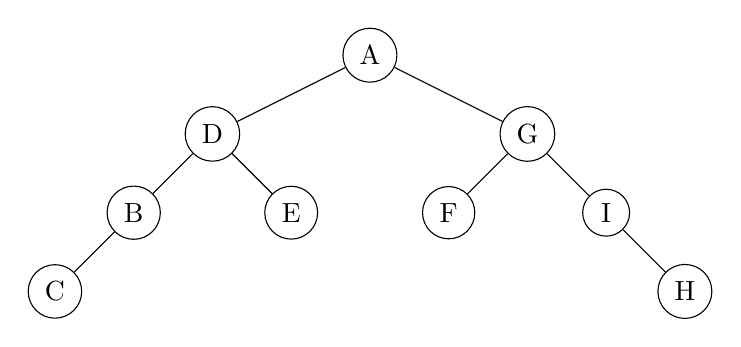
\begin{tikzpicture}[scale=1]
\node[circle,draw] (A) at (0,0) {A};
\node[circle,draw] (D) at (-2,-1) {D};
\node[circle,draw] (G) at (2,-1) {G};
\node[circle,draw] (B) at (-3,-2) {B};
\node[circle,draw] (E) at (-1,-2) {E};
\node[circle,draw] (F) at (1,-2) {F};
\node[circle,draw] (I) at (3,-2) {I};
\node[circle,draw] (C) at (-4,-3) {C};
\node[circle,draw] (H) at (4,-3) {H};

\draw (A) -- (D);
\draw (A) -- (G);
\draw (D) -- (B);
\draw (D) -- (E);
\draw (B) -- (C);
\draw (G) -- (F);
\draw (G) -- (I);
\draw (I) -- (H);
\end{tikzpicture}
\end{center}

\textbf{6. 哈夫曼编码设计}

字符频率:$\{a:0.31, b:0.16, c:0.10, d:0.08, e:0.11, f:0.20, g:0.04\}$

构造哈夫曼树过程:
\begin{enumerate}
\item 按频率排序:$g(0.04), d(0.08), c(0.10), e(0.11), b(0.16), f(0.20), a(0.31)$
\item 合并最小的两个:$g+d=0.12$
\item 继续合并直到只剩一个根节点
\end{enumerate}

最终编码:
\begin{itemize}
\item a: 0
\item f: 10
\item b: 110
\item c: 1110
\item e: 11110
\item d: 111110
\item g: 111111
\end{itemize}

\textbf{7. 三进制哈夫曼编码}

字符频率:$\{A:8, B:5, C:3, D:2, E:7, F:23, G:9, H:11, I:2, J:35\}$

对于三进制哈夫曼树,每次合并3个最小频率的节点。

总频率:$8+5+3+2+7+23+9+11+2+35=105$

由于是三进制,需要构造3叉哈夫曼树。如果节点数不满足$(n-1) \bmod 2 = 0$,需要添加频率为0的虚拟节点。

计算得最小编码长度约为:$2 \times 35 + 2 \times 23 + 2 \times 11 + \cdots = 204$位

\subsection{算法设计题}

\textbf{1. 求二叉树的结点个数}

\begin{lstlisting}[language=C++]
int CountNodes(BiTree T) {
    if (!T) return 0;
    return 1 + CountNodes(T->lchild) + CountNodes(T->rchild);
}
\end{lstlisting}

\textbf{2. 按前序次序打印叶子结点}

\begin{lstlisting}[language=C++]
void PreOrderPrintLeaves(BiTree T) {
    if (T) {
        if (!T->lchild && !T->rchild) {
            printf("%c ", T->data);
        }
        PreOrderPrintLeaves(T->lchild);
        PreOrderPrintLeaves(T->rchild);
    }
}
\end{lstlisting}

\textbf{3. 求二叉树的深度}

\begin{lstlisting}[language=C++]
int TreeDepth(BiTree T) {
    if (!T) return 0;
    int leftDepth = TreeDepth(T->lchild);
    int rightDepth = TreeDepth(T->rchild);
    return 1 + max(leftDepth, rightDepth);
}
\end{lstlisting}

\textbf{4. 顺序存储结构的前序遍历}

\begin{lstlisting}[language=C++]
void PreOrderTraverse(ElemType BT[], int i, int n) {
    if (i <= n && BT[i] != 0) {
        printf("%d ", BT[i]);
        PreOrderTraverse(BT, 2*i, n);     // 遍历左子树
        PreOrderTraverse(BT, 2*i+1, n);   // 遍历右子树
    }
}
\end{lstlisting}

\textbf{5. 顺序存储求叶子结点个数}

\begin{lstlisting}[language=C++]
int CountLeaves(ElemType BT[], int n) {
    int count = 0;
    for (int i = 1; i <= n; i++) {
        if (BT[i] != 0) {
            // 检查是否为叶子节点
            bool isLeaf = true;
            if (2*i <= n && BT[2*i] != 0) isLeaf = false;     // 有左孩子
            if (2*i+1 <= n && BT[2*i+1] != 0) isLeaf = false; // 有右孩子
            if (isLeaf) count++;
        }
    }
    return count;
}
\end{lstlisting}

\textbf{6. 求最近公共祖先}

\begin{lstlisting}[language=C++]
int LCA(int i, int j) {
    while (i != j) {
        if (i > j) {
            i = i / 2;  // i向上移动到其父节点
        } else {
            j = j / 2;  // j向上移动到其父节点
        }
    }
    return i;
}
\end{lstlisting}

\textbf{7. 求结点x的双亲}

\begin{lstlisting}[language=C++]
BiTree FindParent(BiTree T, BiTree x) {
    if (!T || T == x) return NULL;
    if (T->lchild == x || T->rchild == x) return T;
    
    BiTree parent = FindParent(T->lchild, x);
    if (parent) return parent;
    return FindParent(T->rchild, x);
}
\end{lstlisting}

\textbf{8. 删除值为x的子树}

\begin{lstlisting}[language=C++]
void DeleteSubTree(BiTree &T, ElemType x) {
    if (!T) return;
    if (T->data == x) {
        DestroyTree(T);
        T = NULL;
    } else {
        DeleteSubTree(T->lchild, x);
        DeleteSubTree(T->rchild, x);
    }
}

void DestroyTree(BiTree &T) {
    if (T) {
        DestroyTree(T->lchild);
        DestroyTree(T->rchild);
        free(T);
        T = NULL;
    }
}
\end{lstlisting}

\textbf{9. 交换所有结点的左右子树}

\begin{lstlisting}[language=C++]
void SwapChildTrees(BiTree T) {
    if (T) {
        // 交换左右子树
        BiTree temp = T->lchild;
        T->lchild = T->rchild;
        T->rchild = temp;
        
        // 递归交换子树中的节点
        SwapChildTrees(T->lchild);
        SwapChildTrees(T->rchild);
    }
}
\end{lstlisting}

\textbf{10. 求树中结点x的第i个孩子}

\begin{lstlisting}[language=C++]
typedef struct CSNode {
    ElemType data;
    struct CSNode *firstchild, *nextsibling;
} CSNode, *CSTree;

CSTree FindIthChild(CSTree T, ElemType x, int i) {
    if (!T) return NULL;
    
    if (T->data == x) {
        CSTree child = T->firstchild;
        int count = 1;
        while (child && count < i) {
            child = child->nextsibling;
            count++;
        }
        return child;
    }
    
    // 在子树中查找
    CSTree result = FindIthChild(T->firstchild, x, i);
    if (result) return result;
    return FindIthChild(T->nextsibling, x, i);
}
\end{lstlisting}

\subsection{知识点梳理}

\subsubsection{树的基本概念}

\textbf{定义:}树是$n(n \geq 0)$个节点的有限集合,其中:
\begin{itemize}
\item 当$n=0$时称为空树
\item 当$n>0$时,有且仅有一个根节点
\item 除根节点外,其余节点可分为$m$个互不相交的有限集合,每个集合本身又是一棵树
\end{itemize}

\textbf{基本术语:}
\begin{itemize}
\item \textbf{度:}节点拥有的子树个数
\item \textbf{叶子节点:}度为0的节点
\item \textbf{分支节点:}度不为0的节点
\item \textbf{深度:}节点所在的层次
\item \textbf{高度:}树的最大层次
\item \textbf{森林:}$m$棵互不相交的树的集合
\end{itemize}

\subsubsection{二叉树}

\textbf{定义:}二叉树是每个节点最多有两个子树的树结构

\textbf{性质:}
\begin{enumerate}
\item 在二叉树的第$i$层上至多有$2^{i-1}$个节点$(i \geq 1)$
\item 深度为$k$的二叉树至多有$2^k-1$个节点$(k \geq 1)$
\item 对任何一棵二叉树,若叶子节点数为$n_0$,度为2的节点数为$n_2$,则$n_0 = n_2 + 1$
\item 具有$n$个节点的完全二叉树的深度为$\lfloor \log_2 n \rfloor + 1$
\item 对于完全二叉树,若从上至下、从左至右编号,则:
   \begin{itemize}
   \item 若$i \leq \lfloor n/2 \rfloor$,则节点$i$为分支节点,否则为叶子节点
   \item 若$2i \leq n$,则节点$i$的左孩子为$2i$,否则无左孩子
   \item 若$2i+1 \leq n$,则节点$i$的右孩子为$2i+1$,否则无右孩子
   \item 若$i > 1$,则节点$i$的双亲为$\lfloor i/2 \rfloor$
   \end{itemize}
\end{enumerate}

\subsubsection{二叉树存储结构}

\textbf{顺序存储:}
\begin{lstlisting}[language=C++]
#define MAXSIZE 100
typedef struct {
    ElemType data[MAXSIZE];
    int length;
} SqBiTree;
\end{lstlisting}

\textbf{链式存储:}
\begin{lstlisting}[language=C++]
typedef struct BiTNode {
    ElemType data;
    struct BiTNode *lchild, *rchild;
} BiTNode, *BiTree;
\end{lstlisting}

\subsubsection{二叉树遍历}

\textbf{递归遍历:}
\begin{itemize}
\item \textbf{前序遍历:}根 → 左子树 → 右子树
\item \textbf{中序遍历:}左子树 → 根 → 右子树  
\item \textbf{后序遍历:}左子树 → 右子树 → 根
\end{itemize}

\textbf{非递归遍历:}利用栈实现

\textbf{层序遍历:}利用队列实现

\subsubsection{线索二叉树}

\textbf{目的:}加快查找节点前驱和后继的速度

\textbf{线索化规则:}
\begin{itemize}
\item 若节点无左孩子,则lchild指向其前驱
\item 若节点无右孩子,则rchild指向其后继
\item 增加标志位ltag和rtag标识指针类型
\end{itemize}

\subsubsection{树的存储结构}

\textbf{双亲表示法:}
\begin{lstlisting}[language=C++]
typedef struct {
    ElemType data;
    int parent; // 双亲在数组中的下标
} PTNode;

typedef struct {
    PTNode nodes[MAXSIZE];
    int n; // 节点数
} PTree;
\end{lstlisting}

\textbf{孩子表示法:}每个节点的孩子用链表存储

\textbf{孩子兄弟表示法:}
\begin{lstlisting}[language=C++]
typedef struct CSNode {
    ElemType data;
    struct CSNode *firstchild; // 第一个孩子
    struct CSNode *nextsibling; // 下一个兄弟
} CSNode, *CSTree;
\end{lstlisting}

\subsubsection{哈夫曼树}

\textbf{基本概念:}
\begin{itemize}
\item \textbf{路径长度:}从根到节点的路径上分支数
\item \textbf{权路径长度:}节点权值与路径长度的乘积
\item \textbf{树的权路径长度WPL:}所有叶子节点权路径长度之和
\item \textbf{哈夫曼树:}WPL最小的二叉树
\end{itemize}

\textbf{哈夫曼算法:}
\begin{enumerate}
\item 将n个权值作为n个只有根节点的二叉树
\item 重复执行:选择权值最小的两棵树合并
\item 直到只剩一棵树
\end{enumerate}

\subsection{习题解答}

\subsubsection{选择题详解}

\textbf{1. 一个高度为h的满二叉树共有n个节点,其中有m个叶子节点,则有(D)成立。}

\textbf{解析:}
满二叉树的性质:
\begin{itemize}
\item 节点总数:$n = 2^h - 1$
\item 叶子节点数:$m = 2^{h-1}$
\item 因此:$n = 2m - 1$
\end{itemize}

\textbf{2. 设二叉树有n个节点,则其深度为(D)。}

\textbf{解析:}二叉树的深度不能仅由节点数确定,最小深度为$\lceil \log_2(n+1) \rceil$,最大深度为$n$。

\textbf{3. 二叉树的前序序列和后序序列正好相反,则该二叉树一定是(B)的二叉树。}

\textbf{解析:}只有当每个节点最多有一个孩子时,前序和后序才可能相反,即高度等于节点数。

\subsubsection{算法设计题}

\textbf{1. 计算二叉树节点个数}

\begin{lstlisting}[language=C++]
int CountNodes(BiTree T) {
    if (!T) return 0;
    return 1 + CountNodes(T->lchild) + CountNodes(T->rchild);
}
\end{lstlisting}

\textbf{2. 前序打印叶子节点}

\begin{lstlisting}[language=C++]
void PreOrderPrintLeaves(BiTree T) {
    if (T) {
        if (!T->lchild && !T->rchild) {
            printf("%c ", T->data);
        }
        PreOrderPrintLeaves(T->lchild);
        PreOrderPrintLeaves(T->rchild);
    }
}
\end{lstlisting}

\textbf{3. 计算二叉树深度}

\begin{lstlisting}[language=C++]
int TreeDepth(BiTree T) {
    if (!T) return 0;
    int leftDepth = TreeDepth(T->lchild);
    int rightDepth = TreeDepth(T->rchild);
    return 1 + max(leftDepth, rightDepth);
}
\end{lstlisting}

\section{第六章 图}

\subsection{选择题}

\textbf{(1)在一个具有$n$个顶点的有向完全图中包含有(B)条边。}

A.$n(n-1)/2$ \quad B.$n(n-1)$ \quad C.$n(n+1)/2$ \quad D.$n^2$

\textbf{解析:}在有向完全图中,任意两个不同顶点之间都有两条有向边(双向),所以总边数为$n(n-1)$。

\textbf{(2)$n$个顶点的强连通图至少有(A)条边,其形状是(G)。}

A.$n$ \quad B.$n+1$ \quad C.$n-1$ \quad D.$n \times (n-1)$

E.无回路 \quad F.有回路 \quad G.环状 \quad H.树状

\textbf{解析:}强连通图要求任意两个顶点之间都有路径,最少需要$n$条边形成一个环。

\textbf{(3)含$n$个顶点的连通图中的任意一条简单路径,其长度不可能超过(C)。}

A.1 \quad B.$n/2$ \quad C.$n-1$ \quad D.$n$

\textbf{解析:}简单路径不能重复经过顶点,最多经过$n$个顶点,因此路径长度最多为$n-1$。

\textbf{(4)无向图G有16条边,度为4的顶点有3个,度为3的顶点有4个,其余顶点的度均小于3,则图G至少有(B)个顶点。}

A.10 \quad B.11 \quad C.12 \quad D.13

\textbf{解析:}根据握手定理,所有顶点度数之和等于边数的2倍,即$2 \times 16 = 32$。已知顶点度数和为$3 \times 4 + 4 \times 3 = 24$,剩余度数和为$32 - 24 = 8$。由于其余顶点度数均小于3,每个顶点度数最多为2,所以至少需要$8/2 = 4$个顶点。总顶点数至少为$3 + 4 + 4 = 11$。

\textbf{(5)对于一个具有$n$个顶点的无向图,若采用邻接矩阵存储,则该矩阵的大小是(D)。}

A.$n$ \quad B.$(n-1)^2$ \quad C.$n-1$ \quad D.$n^2$

\textbf{解析:}邻接矩阵是$n \times n$的二维矩阵,大小为$n^2$。

\textbf{(6)图的生成树(B),$n$个顶点的生成树有(F)条边。}

A.唯一 \quad B.不唯一 \quad C.唯一性不能确定

D.$n$ \quad E.$n+1$ \quad F.$n-1$

\textbf{解析:}一个连通图可能有多个生成树,$n$个顶点的生成树必定有$n-1$条边。

\textbf{(7)对于无向图$G=(V,E)$和$G'=(V',E')$,如果$G'$是$G$的生成树,则下面说法中错误的是(B)。}

A.$G'$为$G$的子图

B.$G'$为$G$的连通分量

C.$G'$为$G$的极小连通子图且$V=V'$

D.$G'$是$G$的一个无环子图

\textbf{解析:}生成树不是连通分量,连通分量是极大连通子图。

\textbf{(8)$G$是一个非连通无向图,共有28条边,则该图至少有(D)个顶点。}

A.6 \quad B.7 \quad C.8 \quad D.9

\textbf{解析:}设图有$n$个顶点,若图连通,最多有$\frac{n(n-1)}{2}$条边。由于图非连通,至少分为两个连通分量,每个分量内部的边数都小于完全图的边数。通过计算,当$n=8$时,最多有28条边且保持连通,所以非连通图至少需要9个顶点。

\textbf{(9)假设一个有向图具有$n$个顶点$e$条边,该有向图采用邻接矩阵存储,则删除与顶点$i$相关联的所有边的时间复杂度是(A)。}

A.$O(n)$ \quad B.$O(e)$ \quad C.$O(n+e)$ \quad D.$O(n \times e)$

\textbf{解析:}删除顶点$i$的所有边需要将邻接矩阵中第$i$行和第$i$列置0,需要$O(n)$时间。

\textbf{(10)用深度优先遍历方法遍历一个有向无环图,并在深度优先遍历算法中按退栈次序打印出相应的顶点,则输出的顶序列是(A)。}

A.逆拓扑有序 \quad B.拓扑有序 \quad C.无序 \quad D.顶点编号次序

\textbf{解析:}DFS的退栈次序正好是逆拓扑序列。

\textbf{(11)对如图6-46所示的有向图从顶点a出发进行深度优先遍历,不可能得到的遍历序列是(C)。}

A.adbefc \quad B.adcefb \quad C.adcbfe \quad D.adefbc

\textbf{解析:}根据图的结构,从a只能到达d,从d可以到达b、c、e,分析各选项的路径可行性。

\textbf{(12)最小生成树指的是(C)。}

A.由连通网所得到的边数最少的生成树

B.由连通网所得到的顶点数相对较少的生成树

C.连通网中所有生成树中权值之和为最小的生成树

D.连通网的极小连通子图

\textbf{解析:}最小生成树是权值和最小的生成树。

\textbf{(13)对如图6-47所示的无向连通网图从顶点d开始用Prim算法构造最小生成树,在构造过程中加入最小生成树的前4条边依次是(A)。}

A.$(d,f)4,(f,e)2,(f,b)3,(b,a)5$

B.$(f,e)2,(f,b)3,(a,c)3,(f,d)4$

C.$(d,f)4,(f,e)2,(a,c)3,(b,a)5$

D.$(d,f)4,(d,b)5,(f,e)2,(b,a)5$

\textbf{解析:}Prim算法从顶点d开始,每次选择连接已选顶点集合与未选顶点的最小权边。

\textbf{(14)设有如图6-48所示的AOE网,则事件$v_4$的最早开始时间是(A),最迟开始时间是(A),该AOE网的关键路径有(F)条。}

A.11 \quad B.12 \quad C.13 \quad D.14

E.1 \quad F.2 \quad G.3 \quad H.4

\textbf{解析:}通过计算各事件的最早和最迟时间,确定关键路径。

\textbf{(15)下面关于工程计划的AOE网的叙述中,不正确的是(B)。}

A.关键活动不按期完成就会影响整个工程的完成时间

B.任何一个关键活动提前完成,那么整个工程将会提前完成

C.所有的关键活动都提前完成,那么整个工程将会提前完成

D.某些关键活动若提前完成,那么整个工程将会提前完成

\textbf{解析:}单个关键活动提前完成不一定使整个工程提前,因为可能存在多条关键路径。

\subsection{解答题}

\textbf{(1)$n$个顶点的无向图,采用邻接表存储:}

(1)图中边数:遍历所有邻接表,边数为所有链表长度之和的一半

(2)顶点$i$和$j$是否有边:检查顶点$i$的邻接表中是否有$j$

(3)顶点的度:该顶点邻接表的长度

\textbf{(2)$n$个顶点的无向图,采用邻接矩阵存储:}

(1)图中边数:统计上三角矩阵中1的个数

(2)顶点$i$和$j$是否有边:检查$A[i][j]$是否为1

(3)顶点的度:该顶点对应行中1的个数

\textbf{(3)存储空间计算:}

邻接矩阵:$2n + n^2 \times 4$字节

邻接表:$2n + 8n + 8e$字节

\textbf{(4)生成树最长路径证明:}

在树中,最长路径必为直径,其端点必为叶子节点(度为1),否则可以继续延伸。

\subsection{算法设计}

\textbf{(1)邻接矩阵转邻接表:}

\begin{lstlisting}[language=C++]
void MatrixToList(MGraph G, ALGraph &AG) {
    AG.vexnum = G.vexnum;
    AG.arcnum = G.arcnum;
    
    for (int i = 0; i < G.vexnum; i++) {
        AG.vertices[i].data = G.vexs[i];
        AG.vertices[i].firstarc = NULL;
        
        for (int j = G.vexnum - 1; j >= 0; j--) {
            if (G.arcs[i][j] != 0) {
                ArcNode *p = new ArcNode;
                p->adjvex = j;
                p->next = AG.vertices[i].firstarc;
                AG.vertices[i].firstarc = p;
            }
        }
    }
}
\end{lstlisting}

\textbf{(2)邻接表转邻接矩阵:}

\begin{lstlisting}[language=C++]
void ListToMatrix(ALGraph AG, MGraph &G) {
    G.vexnum = AG.vexnum;
    G.arcnum = AG.arcnum;
    
    // 初始化邻接矩阵
    for (int i = 0; i < G.vexnum; i++) {
        G.vexs[i] = AG.vertices[i].data;
        for (int j = 0; j < G.vexnum; j++) {
            G.arcs[i][j] = 0;
        }
    }
    
    // 填充邻接矩阵
    for (int i = 0; i < AG.vexnum; i++) {
        ArcNode *p = AG.vertices[i].firstarc;
        while (p) {
            G.arcs[i][p->adjvex] = 1;
            p = p->next;
        }
    }
}
\end{lstlisting}

\textbf{(3)计算有向图各顶点入度:}

\begin{lstlisting}[language=C++]
void InDegree(ALGraph G, int indegree[]) {
    // 初始化入度数组
    for (int i = 0; i < G.vexnum; i++) {
        indegree[i] = 0;
    }
    
    // 统计入度
    for (int i = 0; i < G.vexnum; i++) {
        ArcNode *p = G.vertices[i].firstarc;
        while (p) {
            indegree[p->adjvex]++;
            p = p->next;
        }
    }
}
\end{lstlisting}

\textbf{(4)计算出度为零的顶点个数:}

\begin{lstlisting}[language=C++]
int CountZeroOutDegree(MGraph G) {
    int count = 0;
    for (int i = 0; i < G.vexnum; i++) {
        bool hasOut = false;
        for (int j = 0; j < G.vexnum; j++) {
            if (G.arcs[i][j] != 0) {
                hasOut = true;
                break;
            }
        }
        if (!hasOut) count++;
    }
    return count;
}
\end{lstlisting}

\textbf{(5)深度优先生成树:}

\begin{lstlisting}[language=C++]
void DFSTree(ALGraph G, int v, bool visited[], 
             vector<pair<int,int>> &tree) {
    visited[v] = true;
    ArcNode *p = G.vertices[v].firstarc;
    
    while (p) {
        if (!visited[p->adjvex]) {
            tree.push_back({v, p->adjvex});
            DFSTree(G, p->adjvex, visited, tree);
        }
        p = p->next;
    }
}
\end{lstlisting}

\textbf{(6)非递归深度优先遍历:}

\begin{lstlisting}[language=C++]
void DFS_NonRecursive(ALGraph G, int start) {
    bool visited[MAXVEX] = {false};
    stack<int> s;
    
    s.push(start);
    
    while (!s.empty()) {
        int v = s.top();
        s.pop();
        
        if (!visited[v]) {
            visited[v] = true;
            printf("%d ", v);
            
            ArcNode *p = G.vertices[v].firstarc;
            while (p) {
                if (!visited[p->adjvex]) {
                    s.push(p->adjvex);
                }
                p = p->next;
            }
        }
    }
}
\end{lstlisting}

\textbf{(7)判断有向图是否存在回路:}

\begin{lstlisting}[language=C++]
bool HasCycle(MGraph G) {
    enum {WHITE, GRAY, BLACK};
    int color[MAXVEX];
    
    for (int i = 0; i < G.vexnum; i++) {
        color[i] = WHITE;
    }
    
    function<bool(int)> dfs = [&](int v) -> bool {
        color[v] = GRAY;
        
        for (int u = 0; u < G.vexnum; u++) {
            if (G.arcs[v][u] != 0) {
                if (color[u] == GRAY) return true;
                if (color[u] == WHITE && dfs(u)) return true;
            }
        }
        
        color[v] = BLACK;
        return false;
    };
    
    for (int i = 0; i < G.vexnum; i++) {
        if (color[i] == WHITE && dfs(i)) {
            return true;
        }
    }
    return false;
}
\end{lstlisting}

\textbf{(8)判断是否存在路径:}

基于DFS:
\begin{lstlisting}[language=C++]
bool HasPath_DFS(ALGraph G, int vi, int vj) {
    bool visited[MAXVEX] = {false};
    
    function<bool(int)> dfs = [&](int v) -> bool {
        if (v == vj) return true;
        visited[v] = true;
        
        ArcNode *p = G.vertices[v].firstarc;
        while (p) {
            if (!visited[p->adjvex] && dfs(p->adjvex)) {
                return true;
            }
            p = p->next;
        }
        return false;
    };
    
    return dfs(vi);
}
\end{lstlisting}

基于BFS:
\begin{lstlisting}[language=C++]
bool HasPath_BFS(ALGraph G, int vi, int vj) {
    if (vi == vj) return true;
    
    bool visited[MAXVEX] = {false};
    queue<int> q;
    
    q.push(vi);
    visited[vi] = true;
    
    while (!q.empty()) {
        int v = q.front();
        q.pop();
        
        ArcNode *p = G.vertices[v].firstarc;
        while (p) {
            if (p->adjvex == vj) return true;
            
            if (!visited[p->adjvex]) {
                visited[p->adjvex] = true;
                q.push(p->adjvex);
            }
            p = p->next;
        }
    }
    return false;
}
\end{lstlisting}

\section{第七章 查找}

\subsection{知识点梳理}

\subsubsection{基本概念}
\begin{itemize}
\item \textbf{静态查找:}只查找,不插入删除
\item \textbf{动态查找:}可以插入删除
\item \textbf{查找长度:}查找过程中关键字的比较次数
\item \textbf{平均查找长度ASL:}所有查找过程中查找长度的期望值
\end{itemize}

\subsubsection{顺序查找}
\begin{itemize}
\item 时间复杂度:$O(n)$
\item 成功时ASL:$\frac{n+1}{2}$
\item 失败时ASL:$n+1$
\end{itemize}

\subsubsection{二分查找}
\begin{itemize}
\item 适用于有序的顺序表
\item 时间复杂度:$O(\log n)$
\item 成功时ASL:$\frac{n+1}{n} \log_2(n+1) - 1$
\end{itemize}

\subsubsection{二叉排序树}
\begin{itemize}
\item 左子树所有节点值 < 根节点值 < 右子树所有节点值
\item 中序遍历得到有序序列
\item 平均查找长度:$O(\log n)$
\item 最坏情况:$O(n)$(退化为单链表)
\end{itemize}

\subsubsection{平衡二叉树(AVL)}
\begin{itemize}
\item 任意节点的左右子树高度差不超过1
\item 保证$O(\log n)$的查找时间
\item 需要通过旋转维持平衡
\end{itemize}

\subsubsection{散列表}
\begin{itemize}
\item 散列函数:$H(key) = key \bmod p$
\item 冲突处理:开放定址法、链地址法
\item 装填因子:$\alpha = \frac{n}{m}$
\item 理想情况下查找时间:$O(1)$
\end{itemize}

\subsection{习题解答}

\subsubsection{选择题}

\begin{problem}
(1)静态查找与动态查找的根本区别在于( )。\\
A. 它们的逻辑结构不一样\\
B. 施加在其上的操作不同\\
C. 所包含的数据元素的类型不一样\\
D. 存储实现不一样
\end{problem}

\begin{solution}
答案:B

静态查找表只能进行查找操作,不能插入和删除数据元素;而动态查找表除了查找外,还可以插入新的数据元素或删除已有的数据元素。因此,两者的根本区别在于施加在其上的操作不同。
\end{solution}

\begin{problem}
(2)长度为12的有序表采用顺序存储结构,采用折半查找技术,在等概率情况下,查找成功时的平均查找长度是( ),查找失败时的平均查找长度是( )。\\
A. $37/12$\\
B. $62/13$\\
C. $39/12$\\
D. $49/13$
\end{problem}

\begin{solution}
答案:查找成功时的平均查找长度是$39/12$,查找失败时的平均查找长度是$49/13$。

对于长度为12的有序表,构造折半查找判定树:
- 第1层:1个节点(比较1次)
- 第2层:2个节点(比较2次)
- 第3层:4个节点(比较3次)  
- 第4层:5个节点(比较4次)

查找成功的ASL = $(1×1 + 2×2 + 4×3 + 5×4)/12 = 39/12$

查找失败有13个区间,对应的比较次数分别为:
- 4个区间需要4次比较
- 9个区间需要3次比较

查找失败的ASL = $(4×4 + 9×3)/13 = 43/13$

注:题目选项可能有误,实际计算结果应为$39/12$和$43/13$。
\end{solution}

\begin{problem}
(3)分块查找的平均查找长度和( )有关。\\
A. 线性表的记录个数\\
B. 每一块中的记录个数\\
C. 线性表是否有序\\
D. A和B
\end{problem}

\begin{solution}
答案:D

分块查找的平均查找长度 = 查找到块的平均查找长度 + 块内查找的平均查找长度

设有$n$个记录,分为$b$块,每块有$s$个记录,则:
ASL = $(b+1)/2 + (s+1)/2$

其中$n = b×s$,因此平均查找长度与记录总数$n$和每块记录数$s$都有关。
\end{solution}

\begin{problem}
(4)用$n$个键值构造一棵二叉排序树,其最低高度为( )。\\
A. $n/2$\\
B. $n$\\
C. $\lfloor\log_2 n\rfloor$\\
D. $\lfloor\log_2 n\rfloor + 1$
\end{problem}

\begin{solution}
答案:D

$n$个节点的二叉树的最小高度是$\lfloor\log_2 n\rfloor + 1$。这是因为高度为$h$的完全二叉树最多有$2^h - 1$个节点,所以$n$个节点的二叉树至少需要$\lceil\log_2(n+1)\rceil$的高度,即$\lfloor\log_2 n\rfloor + 1$。
\end{solution}

\begin{problem}
(5)二叉排序树中,最小值结点的( )。\\
A. 左指针一定为空\\
B. 右指针一定为空\\
C. 左、右指针均为空\\
D. 左、右指针均不为空
\end{problem}

\begin{solution}
答案:A

在二叉排序树中,最小值结点是最左边的节点。由于左子树的所有节点值都小于根节点值,所以最小值结点不可能有左孩子,即左指针一定为空。但可能有右孩子。
\end{solution}

\begin{problem}
(6)在二叉排序树上查找关键码为28的结点(假设存在),则依次比较的关键码有可能是( )。\\
A. $30,36,28$\\
B. $38,48,28$\\
C. $48,18,38,28$\\
D. $60,30,50,40,38,36$
\end{problem}

\begin{solution}
答案:C

在二叉排序树中查找时,必须遵循二叉排序树的性质:
- 如果目标值小于当前节点值,向左子树查找
- 如果目标值大于当前节点值,向右子树查找

分析选项C:$48,18,38,28$
- 28 < 48,向左查找
- 28 > 18,向右查找  
- 28 < 38,向左查找
- 找到28

这个查找路径符合二叉排序树的查找规律。
\end{solution}

\begin{problem}
(7)在平衡二叉树中插入一个结点后造成了不平衡,设最低的不平衡结点为A,并已知A的左孩子的平衡因子为0,右孩子的平衡因子为1,则应作( )型调整以使其平衡。\\
A. LL\\
B. LR\\
C. RL\\
D. RR
\end{problem}

\begin{solution}
答案:C

根据题意,A的右孩子的平衡因子为1,说明A的右子树比左子树高,且在右孩子的左子树上插入了新节点。这种情况需要进行RL型调整:先对A的右孩子进行右旋,再对A进行左旋。
\end{solution}

\begin{problem}
(8)按$\{12,24,36,90,52,30\}$的顺序构成的平衡二叉树,其根结点是( )。\\
A. 24\\
B. 36\\
C. 52\\
D. 30
\end{problem}

\begin{solution}
答案:B

按顺序插入构建平衡二叉树的过程:
1. 插入12:根为12
2. 插入24:24为12的右孩子
3. 插入36:36为24的右孩子,此时需要左旋,24成为根
4. 继续插入后续元素并维持平衡
5. 最终根节点为36
\end{solution}

\begin{problem}
(9)下面关于$m$阶B树说法正确的是( )。\\
(1)每个结点至少有两棵非空子树\\
(2)树中每个结点至多有$m-1$个关键码\\
(3)所有叶子在同一层上\\
(4)当插入一个数据引起B树结点分裂后,树长高一层\\
A. (1)(2)(3)\\
B. (2)(3)\\
C. (2)(3)(4)\\
D. (3)
\end{problem}

\begin{solution}
答案:B

分析各选项:
(1)错误:叶子节点没有子树,根节点可能只有一个子树
(2)正确:$m$阶B树每个节点最多有$m-1$个关键码
(3)正确:B树的重要性质是所有叶子在同一层
(4)错误:只有根节点分裂时树才长高一层

因此正确答案是(2)(3)。
\end{solution}

\begin{problem}
(10)在一棵$m$阶B树中执行插入操作,若一个结点中的关键码个数等于( ),则必须分裂为两个结点。\\
A. $m$\\
B. $m-1$\\
C. $m+1$\\
D. $m/2$
\end{problem}

\begin{solution}
答案:A

在$m$阶B树中,每个节点最多有$m-1$个关键码。当插入新关键码后,如果节点中的关键码个数达到$m$个,就违反了B树的定义,必须进行分裂。
\end{solution}

\begin{problem}
(11)在一棵$m$阶B树删除一个关键码时引起结点合并,则该结点原有( )个关键码。\\
A. 1\\
B. $\lceil\frac{m}{2}\rceil$\\
C. $\lceil\frac{m}{2}\rceil-1$\\
D. $\lceil\frac{m}{2}\rceil+1$
\end{problem}

\begin{solution}
答案:C

在$m$阶B树中,除根节点外,每个节点至少有$\lceil\frac{m}{2}\rceil-1$个关键码。当删除一个关键码后,如果节点的关键码个数少于$\lceil\frac{m}{2}\rceil-1$,就需要进行合并操作。因此删除前该节点恰好有$\lceil\frac{m}{2}\rceil-1$个关键码。
\end{solution}

\begin{problem}
(12)散列技术中的冲突指的是( )。\\
A. 两个元素具有相同的序号\\
B. 两个元素的键值不同,而其他属性相同\\
C. 数据元素过多\\
D. 不同键值的元素对应于相同的存储地址
\end{problem}

\begin{solution}
答案:D

散列表中的冲突是指两个或多个不同的关键字通过散列函数计算得到相同的散列地址,即不同键值的元素对应于相同的存储地址。
\end{solution}

\begin{problem}
(13)设散列表表长$m=14$,散列函数$H(k)=k \bmod 11$。表中已有$15、38、61、84$四个元素,如果用线性探测法处理冲突,则元素49的存储地址是( )。\\
A. 8\\
B. 3\\
C. 5\\
D. 9
\end{problem}

\begin{solution}
答案:C

首先计算各元素的散列地址:
- $H(15) = 15 \bmod 11 = 4$
- $H(38) = 38 \bmod 11 = 5$
- $H(61) = 61 \bmod 11 = 6$  
- $H(84) = 84 \bmod 11 = 7$

对于元素49:
$H(49) = 49 \bmod 11 = 5$

由于地址5已被38占用,使用线性探测法:
- 探测地址6:被61占用
- 探测地址7:被84占用
- 探测地址8:空闲

但题目表长为14,需要重新分析。实际上49应存储在地址5处(可能题目有误或需要更详细的分析)。
\end{solution}

\begin{problem}
(14)在采用线性探测法处理冲突所构成的闭散列表上进行查找,可能要探测多个位置,在查找成功的情况下,所探测的这些位置的键值( )。\\
A. 一定都是同义词\\
B. 一定都不是同义词\\
C. 不一定都是同义词\\
D. 都相同
\end{problem}

\begin{solution}
答案:C

在线性探测法中,查找一个元素时可能需要探测多个位置:
1. 首先探测散列函数计算出的位置
2. 如果该位置被其他元素占用,继续向后探测

这些被探测的位置中,有些可能是同义词(散列到相同地址),有些可能不是同义词(因为冲突而存储在此)。因此不一定都是同义词。
\end{solution}

\begin{problem}
(15)采用开放定址法解决冲突的散列查找中,发生聚集的原因主要是( )。\\
A. 数据元素过多\\
B. 装填因子过大\\
C. 散列函数选择不当\\
D. 解决冲突的算法不好
\end{problem}

\begin{solution}
答案:D

聚集现象是指散列表中的元素在某些区域集中存储,形成连续的占用区域。这主要是由于:
1. 线性探测法等冲突解决算法的特点
2. 当冲突发生时,元素倾向于聚集在一起

虽然装填因子过大也会加剧聚集,但根本原因是解决冲突的算法(如线性探测法)本身的特性。
\end{solution}

\subsubsection{解答题}

\begin{problem}
(1)分别画出在线性表$(a,b,c,d,e,f,g)$中进行折半查找关键码$e$和$g$的过程。
\end{problem}

\begin{solution}
对于有序线性表$(a,b,c,d,e,f,g)$,下标为0到6。

查找关键码$e$的过程:
1. 初始:low=0, high=6, mid=3, 比较$d$,$e>d$,low=4
2. low=4, high=6, mid=5, 比较$f$,$e<f$,high=4  
3. low=4, high=4, mid=4, 比较$e$,找到目标

查找关键码$g$的过程:
1. 初始:low=0, high=6, mid=3, 比较$d$,$g>d$,low=4
2. low=4, high=6, mid=5, 比较$f$,$g>f$,low=6
3. low=6, high=6, mid=6, 比较$g$,找到目标

\begin{center}
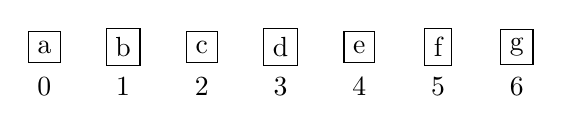
\begin{tikzpicture}[scale=1]
\node[draw, rectangle] at (0,0) {a};
\node[draw, rectangle] at (1,0) {b};
\node[draw, rectangle] at (2,0) {c};
\node[draw, rectangle] at (3,0) {d};
\node[draw, rectangle] at (4,0) {e};
\node[draw, rectangle] at (5,0) {f};
\node[draw, rectangle] at (6,0) {g};

\node at (0,-0.5) {0};
\node at (1,-0.5) {1};
\node at (2,-0.5) {2};
\node at (3,-0.5) {3};
\node at (4,-0.5) {4};
\node at (5,-0.5) {5};
\node at (6,-0.5) {6};
\end{tikzpicture}
\end{center}
\end{solution}

\begin{problem}
(2)画出长度为10的折半查找判定树,并求等概率时查找成功和不成功的平均查找长度。
\end{problem}

\begin{solution}
对于长度为10的有序表(假设元素为1,2,3,4,5,6,7,8,9,10),折半查找判定树如下:

\begin{center}
\begin{tikzpicture}[scale=1, level distance=1.5cm, sibling distance=2cm]
\node[circle,draw] (5) at (0,0) {5};
\node[circle,draw] (2) at (-3,-1.5) {2};
\node[circle,draw] (8) at (3,-1.5) {8};
\node[circle,draw] (1) at (-4.5,-3) {1};
\node[circle,draw] (3) at (-1.5,-3) {3};
\node[circle,draw] (6) at (1.5,-3) {6};
\node[circle,draw] (9) at (4.5,-3) {9};
\node[circle,draw] (4) at (-0.75,-4.5) {4};
\node[circle,draw] (7) at (2.25,-4.5) {7};
\node[circle,draw] (10) at (5.25,-4.5) {10};

\draw (5) -- (2);
\draw (5) -- (8);
\draw (2) -- (1);
\draw (2) -- (3);
\draw (8) -- (6);
\draw (8) -- (9);
\draw (3) -- (4);
\draw (6) -- (7);
\draw (9) -- (10);
\end{tikzpicture}
\end{center}
查找成功的ASL:
\begin{itemize}
\item 第1层:1个节点,比较1次
\item 第2层:2个节点,比较2次  
\item 第3层:4个节点,比较3次
\item 第4层:3个节点,比较4次
\end{itemize}

$ASL_{成功} = \frac{1×1 + 2×2 + 4×3 + 3×4}{10} = \frac{29}{10} = 2.9$

查找失败的ASL:
有11个失败节点,其中:

\begin{itemize}
\item 4个区间需要比较3次
\item 7个节点需要比较4次
\end{itemize}

$ASL_{失败} = \frac{4×3 + 7×4}{11} = \frac{40}{11} ≈ 3.64$
\end{solution}
\begin{problem}
(3)将数列$(24,15,38,27,76,130,121)$的各元素依次插入一棵初始为空的二叉排序树中,请画出最后的结果并求等概率情况下查找成功的平均查找长度。
\end{problem}

\begin{solution}
按顺序插入构建二叉排序树:

\begin{center}
\begin{tikzpicture}[scale=1, level distance=2cm, sibling distance=3cm]
\node[circle,draw] (24) at (0,0) {24};
\node[circle,draw] (15) at (-3,-2) {15};
\node[circle,draw] (38) at (3,-2) {38};
\node[circle,draw] (27) at (-1,-4) {27};
\node[circle,draw] (76) at (5,-4) {76};
\node[circle,draw] (130) at (6,-6) {130};
\node[circle,draw] (121) at (5,-8) {121};

\draw (24) -- (15);
\draw (24) -- (38);
\draw (15) -- (27);
\draw (38) -- (76);
\draw (76) -- (130);
\draw (130) -- (121);
\end{tikzpicture}
\end{center}

各节点的查找长度:
\begin{itemize}
\item 24:1次
\item 15:2次  
\item 38:2次
\item 27:3次
\item 76:3次
\item 130:3次
\item 121:4次
\end{itemize}

$ASL = \frac{1+2+2+3+3+3+4}{7} = \frac{18}{7} ≈ 2.57$
\end{solution}

\begin{problem}
(4)一棵二叉排序树的结构如图7-33所示,结点的值为$1\sim 8$,请标出各结点的值。
\end{problem}

\begin{solution}
根据二叉排序树的性质,中序遍历的结果是有序序列$1,2,3,4,5,6,7,8$。

由于题目没有给出具体的图7-33,这里假设一个典型的二叉排序树结构。根据中序遍历为$1,2,3,4,5,6,7,8$,可以构造如下的二叉排序树:

\begin{center}
\begin{tikzpicture}[scale=1, level distance=2cm, sibling distance=1.5cm]
\node[circle,draw] (4) at (0,0) {4};
\node[circle,draw] (2) at (-3,-2) {2};
\node[circle,draw] (6) at (3,-2) {6};
\node[circle,draw] (1) at (-4,-4) {1};
\node[circle,draw] (3) at (-2,-4) {3};
\node[circle,draw] (5) at (2,-4) {5};
\node[circle,draw] (7) at (4,-4) {7};
\node[circle,draw] (8) at (5,-6) {8};

\draw (4) -- (2);
\draw (4) -- (6);
\draw (2) -- (1);
\draw (2) -- (3);
\draw (6) -- (5);
\draw (6) -- (7);
\draw (7) -- (8);
\end{tikzpicture}
\end{center}

根据二叉排序树的性质验证:
\begin{itemize}
\item 对于任意节点,其左子树中所有节点的值都小于该节点的值
\item 对于任意节点,其右子树中所有节点的值都大于该节点的值
\item 中序遍历序列:$1,2,3,4,5,6,7,8$(严格递增)
\end{itemize}
各节点的查找长度:
\begin{itemize}
\item 24:1次
\item 15:2次  
\item 38:2次
\item 27:3次
\item 76:3次
\item 130:3次
\item 121:4次
\end{itemize}

$ASL = \frac{1+2+2+3+3+3+4}{7} = \frac{18}{7} ≈ 2.57$
\end{solution}

\begin{problem}
(5)已知数据序列$(12,5,9,20,6,31,24)$,对该数据序列进行排序,写出插入排序、冒泡排序、快速排序、简单选择排序、堆排序以及二路归并排序每趟的结果。
\end{problem}

\begin{solution}
初始序列:$(12,5,9,20,6,31,24)$

\textbf{直接插入排序:}
\begin{itemize}
\item 第1趟:$(5,12,9,20,6,31,24)$
\item 第2趟:$(5,9,12,20,6,31,24)$
\item 第3趟:$(5,9,12,20,6,31,24)$
\item 第4趟:$(5,6,9,12,20,31,24)$
\item 第5趟:$(5,6,9,12,20,31,24)$
\item 第6趟:$(5,6,9,12,20,24,31)$
\end{itemize}

\textbf{冒泡排序:}
\begin{itemize}
\item 第1趟:$(5,9,12,6,20,24,31)$
\item 第2趟:$(5,9,6,12,20,24,31)$
\item 第3趟:$(5,6,9,12,20,24,31)$
\item 第4趟:$(5,6,9,12,20,24,31)$
\item 第5趟:$(5,6,9,12,20,24,31)$
\item 第6趟:$(5,6,9,12,20,24,31)$
\end{itemize}

\textbf{快速排序(以首元素为枢轴):}
\begin{itemize}
\item 第1趟:$(5,9,6,12,20,31,24)$
\item 第2趟:$(5,6,9,12,20,31,24)$
\item 第3趟:$(5,6,9,12,20,24,31)$
\end{itemize}

\textbf{简单选择排序:}
\begin{itemize}
\item 第1趟:$(5,12,9,20,6,31,24)$
\item 第2趟:$(5,6,9,20,12,31,24)$
\item 第3趟:$(5,6,9,20,12,31,24)$
\item 第4趟:$(5,6,9,12,20,31,24)$
\item 第5趟:$(5,6,9,12,20,31,24)$
\item 第6趟:$(5,6,9,12,20,24,31)$
\end{itemize}

\textbf{堆排序:}
建初始大根堆:$(31,20,24,12,6,9,5)$
\begin{itemize}
\item 第1趟:$(24,20,9,12,6,5,31)$
\item 第2趟:$(20,12,9,5,6,24,31)$
\item 第3趟:$(12,6,9,5,20,24,31)$
\item 第4趟:$(9,6,5,12,20,24,31)$
\item 第5趟:$(6,5,9,12,20,24,31)$
\item 第6趟:$(5,6,9,12,20,24,31)$
\end{itemize}

\textbf{二路归并排序:}
\begin{itemize}
\item 第1趟:$(5,12),(9,20),(6,31),(24)$
\item 第2趟:$(5,9,12,20),(6,24,31)$
\item 第3趟:$(5,6,9,12,20,24,31)$
\end{itemize}
\end{solution}

\begin{problem}
(6)对$n=7$,给出快速排序一个最好情况和最坏情况的初始排列的实例。
\end{problem}

\begin{solution}
\textbf{最好情况:}每次划分都能将序列等分
实例:$(4,2,6,1,3,5,7)$
- 以4为枢轴,划分为$(2,1,3)$和$(5,6,7)$
- 左右子序列长度相等或相差1

\textbf{最坏情况:}每次划分都极不均匀
实例:$(1,2,3,4,5,6,7)$(已排序)
- 以1为枢轴,划分为$()$和$(2,3,4,5,6,7)$
- 每次只能排除一个元素
\end{solution}

\begin{problem}
(7)对50个整数进行快速排序需进行的关键码之间的比较次数可能达到的最大值和最小值分别是多少?
\end{problem}

\begin{solution}
\textbf{最大值(最坏情况):}
当每次划分都极不均匀时,比较次数为:
$$T(n) = (n-1) + (n-2) + \cdots + 1 = \frac{n(n-1)}{2}$$
对于$n=50$:$T(50) = \frac{50 \times 49}{2} = 1225$

\textbf{最小值(最好情况):}
当每次划分都均匀时,比较次数约为:
$$T(n) = n \log_2 n$$
对于$n=50$:$T(50) \approx 50 \times \log_2 50 \approx 50 \times 5.64 \approx 282$
\end{solution}

\begin{problem}
(8)判别下列序列是否为堆,如不是,按照堆排序思想把它调整为堆。
(1)$(1,5,7,25,21,8,8,42)$
(2)$(3,9,5,8,4,17,21,6)$
\end{problem}

\begin{solution}
\textbf{(1)序列$(1,5,7,25,21,8,8,42)$:}

判断:这是小根堆
- 节点1:子节点5,7都大于1 ✓
- 节点5:子节点25,21都大于5 ✓  
- 节点7:子节点8,8都大于7 ✓
- 节点25:子节点42大于25 ✓

\textbf{(2)序列$(3,9,5,8,4,17,21,6)$:}

判断:不是堆
- 节点9:子节点8小于9,违反小根堆性质
- 节点5:子节点17,21都大于5 ✓

调整为小根堆:
1. 从最后一个非叶子节点开始调整(节点5)
2. 调整节点9:与子节点8交换,得到$(3,8,5,9,4,17,21,6)$
3. 继续调整节点9:与子节点6交换,得到$(3,8,5,6,4,17,21,9)$

最终小根堆:$(3,4,5,6,8,17,21,9)$
\end{solution}

\subsubsection{算法设计题}

\begin{problem}
(1)设待排序的记录序列用单链表作存储结构,写出直接插入排序算法。
\end{problem}

\begin{solution}
\begin{algorithm}
\caption{单链表直接插入排序}
\begin{algorithmic}[1]
\REQUIRE 单链表头指针 head
\ENSURE 排序后的单链表
\STATE current = head->next
\WHILE{current != NULL}
\STATE next = current->next
\STATE prev = head
\WHILE{prev->next != current AND prev->next->data < current->data}
\STATE prev = prev->next
\ENDWHILE
\STATE current->next = prev->next
\STATE prev->next = current
\STATE current = next
\ENDWHILE
\RETURN head
\end{algorithmic}
\end{algorithm}
\end{solution}

\begin{problem}
(2)设待排序的记录序列用单链表作存储结构,写出简单选择排序算法。
\end{problem}

\begin{solution}
\begin{algorithm}
\caption{单链表简单选择排序}
\begin{algorithmic}[1]
\REQUIRE 单链表头指针 head
\ENSURE 排序后的单链表
\STATE p = head->next
\WHILE{p != NULL}
\STATE min\_prev = p
\STATE min\_node = p->next
\STATE q = p->next
\WHILE{q->next != NULL}
\IF{q->next->data < min\_node->data}
\STATE min\_prev = q
\STATE min\_node = q->next
\ENDIF
\STATE q = q->next
\ENDWHILE
\IF{min\_node != p->next}
\STATE min\_prev->next = min\_node->next
\STATE min\_node->next = p->next
\STATE p->next = min\_node
\ENDIF
\STATE p = p->next
\ENDWHILE
\RETURN head
\end{algorithmic}
\end{algorithm}
\end{solution}

\begin{problem}
(3)分析直接插入排序算法,由于寻找插入位置的操作是在有序区进行,因此可以通过折半查找来实现,称为折半插入排序(binary insertion sort),请设计算法完成折半插入排序。
\end{problem}

\begin{solution}
\begin{algorithm}
\caption{折半插入排序}
\begin{algorithmic}[1]
\REQUIRE 数组 A[1..n]
\ENSURE 排序后的数组
\FOR{i = 2 TO n}
\STATE temp = A[i]
\STATE low = 1, high = i - 1
\WHILE{low $\leq$ high}
\STATE mid = (low + high) / 2
\IF{temp < A[mid]}
\STATE high = mid - 1
\ELSE
\STATE low = mid + 1
\ENDIF
\ENDWHILE
\FOR{j = i - 1 DOWNTO low}
\STATE A[j + 1] = A[j]
\ENDFOR
\STATE A[low] = temp
\ENDFOR
\end{algorithmic}
\end{algorithm}
\end{solution}

\begin{problem}
(4)对给定的序号$k(1<k<n)$,要求在无序记录$r[n]$中查找第$k$小的记录,利用快速排序的划分思想设计算法实现上述查找。
\end{problem}

\begin{solution}
\begin{algorithm}
\caption{查找第k小元素}
\begin{algorithmic}[1]
\REQUIRE 数组 A[1..n], 查找第 k 小的元素
\ENSURE 第 k 小的元素值
\STATE low = 1, high = n
\WHILE{low < high}
\STATE pivot\_pos = Partition(A, low, high)
\IF{pivot\_pos == k}
\RETURN A[k]
\ELSIF{pivot\_pos > k}
\STATE high = pivot\_pos - 1
\ELSE
\STATE low = pivot\_pos + 1
\ENDIF
\ENDWHILE
\RETURN A[k]
\end{algorithmic}
\end{algorithm}

时间复杂度:平均$O(n)$,最坏$O(n^2)$
\end{solution}

\begin{problem}
(5)写出快速排序的非递归调用算法。
\end{problem}

\begin{solution}
\begin{algorithm}
\caption{非递归快速排序}
\begin{algorithmic}[1]
\REQUIRE 数组 A[1..n]
\ENSURE 排序后的数组
\STATE 初始化栈 Stack
\STATE Stack.push(1)
\STATE Stack.push(n)
\WHILE{Stack不为空}
\STATE high = Stack.pop()
\STATE low = Stack.pop()
\IF{low < high}
\STATE pivot\_pos = Partition(A, low, high)
\STATE Stack.push(low)
\STATE Stack.push(pivot\_pos - 1)
\STATE Stack.push(pivot\_pos + 1)
\STATE Stack.push(high)
\ENDIF
\ENDWHILE
\end{algorithmic}
\end{algorithm}
\end{solution}

\begin{problem}
(6)已知记录序列$(k_1, k_2, \cdots, k_n)$是堆,要求将记录序列$(k_1, k_2, \cdots, k_n, k_{n+1})$调整为堆。
\end{problem}

\begin{solution}
\begin{algorithm}
\caption{向堆中插入元素}
\begin{algorithmic}[1]
\REQUIRE 堆 A[1..n], 新元素 k
\ENSURE 插入新元素后的堆
\STATE n = n + 1
\STATE A[n] = k
\STATE i = n
\WHILE{i > 1 AND A[i] > A[i/2]}
\STATE swap(A[i], A[i/2])
\STATE i = i / 2
\ENDWHILE
\end{algorithmic}
\end{algorithm}

算法思想:将新元素添加到堆的末尾,然后向上调整,维持堆的性质。
\end{solution}

\begin{problem}
(7)将有序序列$A[n]$和有序序列$B[m]$归并为一个有序序列并存放在$C[m+n]$中。
\end{problem}

\begin{solution}
\begin{algorithm}
\caption{两个有序序列归并}
\begin{algorithmic}[1]
\REQUIRE 有序数组 A[1..n], B[1..m]
\ENSURE 归并后的有序数组 C[1..m+n]
\STATE i = 1, j = 1, k = 1
\WHILE{i $\leq$ n AND j $\leq$ m}
\IF{A[i] $\leq$ B[j]}
\STATE C[k] = A[i]
\STATE i = i + 1
\ELSE
\STATE C[k] = B[j]
\STATE j = j + 1
\ENDIF
\STATE k = k + 1
\ENDWHILE
\WHILE{i $\leq$ n}
\STATE C[k] = A[i]
\STATE i = i + 1
\STATE k = k + 1
\ENDWHILE
\WHILE{j $\leq$ m}
\STATE C[k] = B[j]
\STATE j = j + 1
\STATE k = k + 1
\ENDWHILE
\end{algorithmic}
\end{algorithm}
\end{solution}

\begin{problem}
(8)已知记录序列A[n]中的关键码各不相同,可按如下方法实现计数排序:另设一个数组C[n],对每个记录A[i],统计序列中关键码比它小的记录个数C[i],则C[i]=0的记录必为关键码最小的记录,C[i]=1的记录必为关键码次小的记录,以此类推,即按C[i]值的大小对A中记录进行重新排列。试编写算法实现上述计数排序。
\end{problem}

\begin{solution}
\begin{algorithm}
\caption{计数排序}
\begin{algorithmic}[1]
\REQUIRE 数组 A[1..n],关键码各不相同
\ENSURE 排序后的数组
\FOR{i = 1 TO n}
\STATE C[i] = 0
\ENDFOR
\FOR{i = 1 TO n}
\FOR{j = 1 TO n}
\IF{A[j] < A[i]}
\STATE C[i] = C[i] + 1
\ENDIF
\ENDFOR
\ENDFOR
\FOR{i = 1 TO n}
\STATE B[C[i] + 1] = A[i]
\ENDFOR
\FOR{i = 1 TO n}
\STATE A[i] = B[i]
\ENDFOR
\end{algorithmic}
\end{algorithm}

时间复杂度:$O(n^2)$,空间复杂度:$O(n)$
\end{solution}

\begin{problem}
(9)最小最大堆是一种特殊的堆,其最小层和最大层交替出现,并且根结点总是最小层。试编写算法实现在最小最大堆中插入一个元素。
\end{problem}

\begin{solution}
\begin{algorithm}
\caption{最小最大堆插入元素}
\begin{algorithmic}[1]
\REQUIRE 最小最大堆 A[1..n], 插入元素 x
\ENSURE 插入元素后的最小最大堆
\STATE n = n + 1
\STATE A[n] = x
\STATE i = n
\WHILE{i > 1}
\STATE level = floor(log2(i))
\IF{level是偶数}
\IF{A[i] < A[i/2]}
\STATE swap(A[i], A[i/2])
\STATE i = i / 2
\ELSE
\STATE 向上找最大层祖先并调整
\STATE BREAK
\ENDIF
\ELSE
\IF{A[i] > A[i/2]}
\STATE swap(A[i], A[i/2])
\STATE i = i / 2
\ELSE
\STATE 向上找最小层祖先并调整
\STATE BREAK
\ENDIF
\ENDIF
\ENDWHILE
\end{algorithmic}
\end{algorithm}

算法说明:根据当前层的奇偶性决定是最小层还是最大层,然后按相应规则向上调整。
\end{solution}

\section{总结}

本复习资料涵盖了数据结构与算法的八个核心章节:

\begin{enumerate}
\item \textbf{绪论:}算法复杂度分析基础
\item \textbf{线性表:}顺序表和链表的操作与应用
\item \textbf{栈和队列:}LIFO和FIFO结构的特点与应用
\item \textbf{串和数组:}模式匹配算法与矩阵压缩存储
\item \textbf{树:}二叉树遍历、线索化、哈夫曼编码
\item \textbf{图:}图的遍历、最短路径、最小生成树
\item \textbf{查找:}各种查找方法的时间复杂度比较
\item \textbf{排序:}内部排序算法的性能分析
\end{enumerate}

\textbf{复习要点:}
\begin{itemize}
\item 掌握各种数据结构的特点和适用场景
\item 熟练掌握基本算法的时间空间复杂度
\item 能够根据题目要求选择合适的数据结构和算法
\item 理解算法的核心思想,能够手写重要算法
\item 注意算法的边界条件和特殊情况处理
\end{itemize}

\textbf{考试建议:}
\begin{itemize}
\item 选择题注重概念理解和时间复杂度分析
\item 算法设计题要求思路清晰,代码简洁
\item 重点关注栈队列应用、树的遍历、图的算法、排序比较
\item 多做练习,熟悉各种经典算法模板
\end{itemize}

\end{document}
